\pdfoutput=1

%=== Packages and Package Configuration ===

\documentclass{l4proj}
\usepackage{amsmath}
\usepackage{algorithm}
\usepackage[noend]{algpseudocode}
\usepackage{microtype}
\usepackage{epigraph}
\usepackage{enumerate}
\usepackage{url}
\usepackage{wrapfig}
\usepackage{breakurl}
\usepackage[breaklinks]{hyperref}
\usepackage{fancyvrb}
\def\UrlBreaks{\do\/\do-}
\usepackage[T1]{fontenc}
\usepackage[utf8]{inputenc}
\usepackage{float}
\usepackage[dvipsnames]{xcolor}
\usepackage{listings}
\hypersetup{
colorlinks,
linkcolor={red!50!black},
citecolor={blue!50!black},
urlcolor={blue!80!black}
}
\setlength{\belowcaptionskip}{17pt plus 3pt minus 2pt}

%=== Custom Macros ===

\newcommand\textttd[1]{\texttt{\detokenize{#1}}}
\newenvironment{halfmini}[1]
{
\begin{minipage}[t]{0.5\textwidth}
\noindent\textbf{\textit{#1}}\\
}
{
\end{minipage}
}
\newcommand\tricksubsection[1]{
\vspace{-1\baselineskip}\subsection{#1}\vspace{-0.3\baselineskip}}

%=== Source Code Listings ===

\DeclareFixedFont{\ttb}{T1}{txtt}{bx}{n}{10}
\DeclareFixedFont{\ttm}{T1}{txtt}{m}{n}{10}
\DeclareFixedFont{\ttbs}{T1}{txtt}{bx}{n}{8}
\DeclareFixedFont{\ttms}{T1}{txtt}{m}{n}{8}
\DeclareFixedFont{\ttbt}{T1}{txtt}{bx}{n}{7}
\DeclareFixedFont{\ttmt}{T1}{txtt}{m}{n}{7}
\definecolor{keyword}{HTML}{8C0D40}
\definecolor{name}{HTML}{000F55}
\newcommand\genericstyle{\lstset{basicstyle=\ttm}}
\newcommand\codeinline[1]{{\genericstyle\lstinline!#1!}}
\newcommand\pythonstyle{\lstset{
language=Python,
basicstyle=\ttm,
otherkeywords={self},
keywordstyle=\ttb\color{keyword},
emph={__init__,ThingDoer,accept_foo_bar,THING_QUOTA,do_thing,Discombobulator,
discombobulate, Discombobulated,func},
emphstyle=\ttb\color{name},
stringstyle=\color{PineGreen},
rulecolor=\color{gray},
showstringspaces=false
}}
\lstnewenvironment{python}[1][]
{
\pythonstyle
\lstset{#1}
}
{}
\newcommand\pythoninline[1]{{\pythonstyle\lstinline!#1!}}
\newcommand\javastyle{\lstset{
language=Java,
basicstyle=\ttm,
otherkeywords={},
keywordstyle=\ttb\color{keyword},
emph={method,MyClass,somePackage,SomeClass,InnerClass,field,String,Integer},
emphstyle=\ttb\color{name},
stringstyle=\color{PineGreen},
rulecolor=\color{gray},
showstringspaces=false
}}
\lstnewenvironment{java}[1][]
{
\javastyle
\lstset{#1}
}
{}
\newcommand\javainline[1]{{\javastyle\lstinline!#1!}}
\newcommand\clojurestyle{\lstset{
language=Lisp,
basicstyle=\ttm,
otherkeywords={defn,defn-,macroexpand,macroexpand-all},
keywordstyle=\ttb\color{keyword},
emph={lib.core,constant,func,get-nil},
emphstyle=\ttb\color{name},
stringstyle=\color{PineGreen},
rulecolor=\color{gray},
showstringspaces=false
}}
\lstnewenvironment{clojure}[1][]
{
\clojurestyle
\lstset{#1}
}
{}
\newcommand\clojureinline[1]{{\clojurestyle\lstinline!#1!}}
\newcommand\clojureinlinedef{
{\clojurestyle\lstset{otherkeywords=def}\lstinline!def!\enspace}}
\newcommand\xmlstyle{\lstset{
language=XML,
basicstyle=\ttm,
otherkeywords={},
keywordstyle=\ttb\color{keyword},
emph={},
emphstyle=\ttb\color{name},
stringstyle=\color{PineGreen},
rulecolor=\color{gray},
showstringspaces=false
}}
\lstnewenvironment{xml}[1][]
{
\xmlstyle
\lstset{#1}
}
{}
\newcommand\xmlinline[1]{{\xmlstyle\lstinline!#1!}}

%=== Before Contents ===

\begin{document}
\title{Automatic Suggestion of Semantic Versioning}
\author{Christian Shtarkov}
\date{\today}
\maketitle

\begin{abstract}
In software development, assigning a version number
to each release is crucial. It allows end users and other developers
to identify that a software package has changed from a previous
iteration. It is especially important when considering libraries and
frameworks, where changes can greatly affect applications built on top
of them. \\ Different policies exist dictating how to assign version
numbers, one of the most popular being \textit{Semantic
Versioning}, where the version gives
information about how exactly the software package has changed.
\\\\
Regardless of
policy, assigning version numbers is typically done manually and
leaves room for human mistakes or deviations from an established
scheme. This project proposes the tool \textit{Autobump} that automatically
inspects changes to a codebase and suggests the next version number
according to semantic versioning.
\end{abstract}

\renewcommand{\abstractname}{Acknowledgments}
\begin{abstract}
I would like to thank my project supervisor -- Dr. Tim Storer -- for
proposing the original idea behind this project and for his continuous
support throughout the academic year.

\noindent Furthermore, I would like to show appreciation for my fellow students
Pavel Dikov, Alex Leet, Hamza Tanveer and David Benicek for the
exchange of ideas that went on during our weekly project supervision
meetings.
\end{abstract}

\educationalconsent

\tableofcontents

%=== Contents ===

\chapter{Introduction}
\pagenumbering{arabic}

\epigraph{The real world is a messy place; there’s nothing we can do
about that but be vigilant.}{Tom Preston-Werner}

This chapter discusses the background of software versioning and more
specifically, semantic versioning of software.
The overall aim of the project is briefly stated and then an outline
of the rest of the document is given.

\section{Background}

\subsection{Software versioning}
Software versioning is the practice of assigning nominal or numerical
identifiers to subsequent iterations of a software package. Every
variant of a piece of software is expected to have a different
(however small the difference) set of functionality, and versioning
allows for finding out how exactly a piece of software is expected to
behave. In practice, all non-trivial software is versioned in one way
or another.

Versioning can have different levels of granularity. Revision control
systems, such as Git or Subversion, allow developers to introduce
small incremental changes to a codebase. After every change, the new
state of the codebase is given a unique identifier and made
recoverable. For example, Subversion assigns a single number to every
revision starting at 1 and increasing in chronological order. This
allows for many productivity-oriented features, such as reverting code
to a previous state, proving that a particular changeset is
responsible for the introduction of a bug, or identifying differences
between divergent branches of the same initial piece of code.

On a macro scale, releases of software packages are also versioned.
Because releases happen much less often than small changes, versions
also change much less often and follow different policies. The de
facto standard are sequence-based schemes where each version
identifier is a tuple consisting of numbers or letters separated by
dots -- e.g. \textit{1.3.2} or \textit{10.6-rc1}. The vast majority of
computer software follows a scheme of this type. It is usually implied
that the further to the left an element of the tuple is, the more
significant it is. What ``significant'' means is not well-defined and
depends on the kind of software that is being versioned. Comparing
versions \textit{5.0} and \textit{6.0} of a Web browser may imply that
the latter is more advanced and has new features, whereas comparing
the same versions of a library may imply that client code using the
former is incompatible with the latter. In general, incrementing
versions in this format follows these rules:
\begin{enumerate}[(i)]
\item Incrementing any non-final element ``resets'' all elements to
the right, i.e. bumping the middle element of \textit{3.5.4} results
in \textit{3.6.0}.
\item Incrementing a version which has a label attached at the end
necessitates either changing the label or droping it, i.e.
\textit{3.5.4-beta} $\rightarrow$ \textit{3.5.4} or \textit{3.5.4-rc1}
$\rightarrow $ \textit{3.5.4-rc2}.
\end{enumerate}

Note that software can be versioned by more than one scheme
simultaneously -- it is a
typical scenario that revision numbers are used by developers
internally and a sequence-based scheme is used for public releases.
Large consumer-facing software with long release cycles, like
operating systems, may use a codename or date-based scheme for
versioning public releases -- e.g. \textit{Ubuntu 14.04 (Trusty Tahr)}
which was released in April of 2014 happens to use both. Those
typically serve a marketing purpose rather than provide any technical
benefit.

\subsection{Semantic versioning}

In software development, it is a widespread practice to leverage
pre-existing code in the form of libraries or
frameworks\footnote{Those are the most common use cases for one piece
of software interfacing with another. The same argument also applies
to conceptually similar use cases, like invoking command-line tools
such as \textit{sed} or \textit{awk} from a script.} to avoid
duplication of effort.

The way that client code usually interacts with these libraries is
through a publically declared interface known as the
\textit{application program interface} (API). In some languages, such
as C, depending on how the vendor provides the library a binary
interface may be used instead (\textit{application binary interface},
ABI), but the general idea of a publically known interface remains the
same. Once client software starts using a library, its further
development is tied to that library, which is now a
\textit{dependency}.

Given that client applications and the libraries they depend on have
separate development cycles, a problem arises in determining whether a
client application is compatible with a different version of the same
library. In software development, backwards compatibility is often
valued because it increases confidence and reduces cost when upgrading
the dependencies of a software package.

Virtually all well-maintained libraries try to provide a \textit{changelog},
which is a compiled list of changes since the last version. They usually
place emphasis on changes that are breaking, as that is most
concerning to developers of client software. Changelogs can be
manually put together, or partially generated by tools such as
\textit{JDiff} \cite{JDiff}. Another common solution is to take a
sequence-based versioning scheme and attach meaning to the positions
in order to measure degree of compatibility.

Semantic versioning \cite{SemanticVersioning} (Semver) is a strict
formalization of such a scheme, where the format and significance of
each position are well-defined:

\begin{center}
$\mathrm{Major.Minor.Patch}(-\mathrm{Prerelease})^?(+\mathrm{Build})^?$
\end{center}

\begin{itemize}
\item \textit{Major} increments when incompatible changes to the
public API have been made and it is possible for interfacing software
to no longer work.
\item \textit{Minor} increments when new features have been added in a
backwards-compatible manner.
\item \textit{Patch} increments when bugs have been fixed in a
backwards-compatible manner.
\item \textit{Prerelease} is an optional label indicating that the
version does not yet meet the compatibility requirements imposed by
the first three numbers.
\item \textit{Build} is another optional label indicating the
corresponding internal version numbers, e.g. the one used by the
revision control system.
\end{itemize}

Semver defines the public API to start at version \textit{1.0.0}.
Versions before that expect the minor and patch version numbers to
change radically and frequently, so their significance is diminished.
For all intents and purposes, software that is at major version
\textit{0} does not yet follow semantic versioning.
If the versioning rules had started applying from the first ever
release of the project, either the developers would be discouraged
from versioning unstable work or version numbers would balloon.

Semver, explicitly or implicitly, is the ``default'' versioning
scheme. This is so by virtue of the fact that in practice the version
numbers of most modern software closely resemble it, at least
syntactically \cite{SemanticVersioning}. As its specification claims,
``these rules are based on but not necessarily limited to pre-existing
widespread common practices in use in both closed and open-source
software.'' It's important to realise that Semver is designed around
the status quo, not the other way around. For example, the Eclipse
project has its own formalised four-segment versioning scheme
\cite{EclipseVersions} which gives slightly different meaning to its
fields than Semver but is very similar nonetheless.

\subsubsection{Benefits}

The Semver specification outlines as motivation that the scheme guards
against a situation known as \textit{dependency hell}. Dependency hell
is when one or both of version lock and version promiscuity occur.
Version lock can happen when dependency requirements are specified too
tightly and the costs of providing the dependencies that satisfy them
start to increase over time. Version promiscuity is the overestimation
of what versions of a dependency are backwards-compatible with whatever
the client application is using at the moment. Specifying that version
``\textit{2.0.0} or better'' is needed can be dangerous if
\textit{2.1.0} stops being backwards-compatible.

Semver alleviates dependency hell by communicating how software has
changed in a new version compared to the previous one by the version
number alone. This allows for a sweet spot in specifying dependency
requirements that are neither too restrictive, nor overly liberal.
It increases confidence and reduces the risk of loss.

This scheme is especially important for automatic dependency
management systems, like ones found in package managers or build
systems. Even if version numbers bore no semantic meaning, humans
would still be able to read changelogs and make decisions about whether
dependencies can be safely upgraded or whether their code should be
changed. However, automated systems are much better informed by
looking at a version number.

\subsubsection{Application}

Semver only provides these benefits when it is applied consistently.
If applied haphazardly, then two versions cannot be compared reliably
and decisions made by simply examining version numbers are risky. If
business-critical software has some dependency which is guaranteed to
follow semantic versioning and a new patch version is released, the
decision to upgrade is a trivial: after all, this patch may resolve
bugs that affect clients. However, this confidence can be unwarranted
even if a single patch release results in a breaking change that
causes the software to fail, or even worse -- behave in unexpected ways.
This leads to a trade-off between confidence and friction when
updating dependencies. This dissertation argues that this situation is
undesirable and can be alleviated.

In practice, semantic versioning is applied poorly. A
study \cite{SemverMaven} of more than 22,000 libraries in the Maven
repository (a dependency management standard that incorporates the use
of semantic versioning) found that there was virtually no difference in the
frequency of breaking changes in major and minor version increments.
It also found that this has a significant impact on client
applications, mostly by causing compilation errors. The study goes on
to suggest that similar results could be found in other ecosystems.

The study suggests that one possible explanation of this low adherence
could be the presence of ``internal'' packages. There is a distinction
between an internal and public API in that the internal is meant for
parts of the library interacting with other parts. The public API is a
superset of that, exposing functionality to end users without allowing
them to meddle in the internals of the program. Internal packages are
designated as such only in name, while they are actually
publically available in order to work around Java's access modifiers.
Although they may not be intended for public use, they are certainly
available to client code. An additional explanation may be that
libraries that poorly follow Semver are intended for use only by the
developers themselves. However, the authors argue, such libraries
should have probably never been released into a public repository.

There is a distinction between an
internal and public API in that the internal is meant for parts of the
library interacting with other parts. The public API is a superset of
that, exposing functionality to end users without allowing them to
meddle in the internals of the program.

Another possible reason might be that some authors are reluctant to follow
semantic versioning, or may be completely unaware that there is a
formalisation of it. Just because a versioning scheme resembles Semver
syntactically does not immediately impart any meaning on the
individual numbers.

Even if authors do intend to follow Semver, their own subjectivity may
get in the way. Developers may be inclined to believe that making a
breaking change to an obscure function that, to their knowledge, is
not being used by anyone is not worthy of being designated as
``breaking''. However, Semver makes no such allowance. It strictly
specifies that any breaking change to the public API warrants
the incrementation of the major version number, regardless of how
insignificant it may appear to be. That applies even for functionality
designated as deprecated in a previous version -- although the same
study found that deprecation annotations were barely used and removal
of functionality is usually sudden.

Even if authors were making a small breaking change to the public API,
and were fully aware that Semver stipulates bumping the major version,
they may still be inclined not to do so. Doing that frequently would
mean the major version number skyrocketing, which for purely
superficial reasons can be undesirable. However, it's important to
realise that this would happen because of development methodology and
not the versioning scheme itself. As the Semver specification
mentions, ``this is a question of responsible development and
foresight. Incompatible changes should not be introduced lightly to
software that has a lot of dependent code.''

\subsubsection{Criticism}

Semantic versioning has received criticism for its inflexible way of
assigning version numbers. Most notably, the essay ``Why Semantic
Versioning Isn't'' \cite{WhySemanticVersioningIsnt} by CoffeeScript
creator Jeremy Ashkenas refers to the scheme as ``romantic
versioning'' because of its alleged failure in real-world scenarios.

The core argument against Semver is that it attempts to compress too
much information into a few numbers. Semver does not acknowledge any
degree of a breaking change, it is a binary decision -- breaking or not.
This fails to reflect the number of affected users, or the difficulty
in porting old software to use the new version of the dependency.

The essay argues that Semver is a false promise, because the majority
of projects do not officially follow it or do so inconsistently.
However, this is a problem of adoption, not something inherent to the
scheme itself.

\clearpage
\section{Aim}

It has been identified that the reluctance or inconsistency of
applying a strict versioning scheme like Semver is a problem in
software engineering that costs development time and obstructs
automated systems like package managers from making decisions about
software upgrades.

This project proposes the automated assignment of version numbers
as a possible solution. The goal is to develop a tool that given a
previous iteration of a project and its version, can automatically
propose the version of the following iteration. This can increase the
level of adherence to semantic versioning in two ways:

\begin{enumerate}[(i)]
\item Taking away the responsibility of providing a new version number
from software developers, leaving less room for human error.
\item Examining the prime source of semantic changes to the project --
the codebase itself.
\end{enumerate}

As an additional requirement, this dissertation examines a
language-agnostic solution to this problem. The resulting tool is then
to be evaluated against the history of real-world libraries across
different languages.

\section{Outline}

The rest of this dissertation is comprised of the following chapters
and appendices:

\noindent Chapter \ref{PreviousWork} -- \textbf{Previous work} \\
Goes into existing projects that to some extent solve the problem
of automatically assigning version numbers and the approaches that
they use.

\noindent Chapter \ref{Approach} -- \textbf{Approach} \\
Lays out the approach that Autobump is going to use for
determining version numbers and the set of features that would make
the tool useful.

\noindent Chapter \ref{Implementation} -- \textbf{Implementation} \\
Discusses how Autobump works in great detail, both internally and
in terms of being exposed to the end user.

\noindent Chapter \ref{Testing} -- \textbf{Testing} \\
Goes into the techniques used to show that Autobump indeed works
as advertised.

\noindent Chapter \ref{Evaluation} -- \textbf{Evaluation} \\
``Replays'' the history of different libraries across the target
languages to find out whether a tool like Autobump would have been
beneficial in their development.

\noindent Chapter \ref{Conclusion} -- \textbf{Conclusion} \\
Summarizes what was accomplished by this project and proposes future
work. \\

\noindent Appendix \ref{AutobumpInPractice} -- \textbf{Running
Autobump in practice} \\\\
\noindent Appendix \ref{ClojurePrimer} -- \textbf{Primer on Clojure} \\\\
\noindent Appendix \ref{AutomatedEvaluationData} -- \textbf{Automated
evaluation data}

\chapter{Previous work}
\label{PreviousWork}

Automatically assigning version numbers is not a new idea and projects
exist that already do that to some extent.
This chapter discusses existing tools that claim to do that. It also
examines the various ways they approach it, why they are not as
successful as it would be expected and draws ideas for how this project
might implement a similar tool.

\section{semantic-release}

\textit{semantic-release} \cite{SemanticRelease} is a Javascript tool
for ``fully automated package publishing''. It can do a range of
functions related to automated publishing of packages in the
Javascript ecosystem through the Node Package Manager, but of interest
are the two ways it can deal with proposing a new version number.

One way is that it tries to interpret Git commit messages and from
that determines what the next version number should be. A minor
(feature) release for example would be indicated by a commit message
of the following format:

\begin{center}
\texttt{feat(pencil): add 'graphiteWidth' option}
\end{center}

This approach suffers from the same drawback as incrementing the
version number manually does -- it has to be done consistently.
Not conforming to the format even once would mean that the tool would
fail to identify that the version should be bumped.

Another way is by employing an additional tool called
\textit{cracks} \cite{Cracks}. According to the official description
``this module can automatically detect breaking changes by running the
test suite of your last-release against the current codebase.''
This is generally a good approach -- ideally
the test suite of the previous version should pass if the new one is
not meant to be a major release. However, it raises some issues.

\begin{itemize}
\item It could be that the library in question has whitebox unit
tests. If they start failing, that does not necessarily constitute a
breaking change\footnote{As far as the public API is concerned. It
could be that the modification of implementation details implies that
the function now has different semantics or purpose. This is really
another view on what is a ``breaking'' change.}, because while the
internal implementation of
those methods may have changed, the public API could still be the
same. Cracks has no way of differentiating blackbox from whitebox
tests unless manually specified.
\item The unit tests may not cover the public API in its entirety.
Modifying the signature of a public method, for example, that's not
covered by the tests may go completely unnoticed.
\item The library may be in a stage of development such that it has no
unit tests, or they cover a very small portion of the public API, yet
the authors still want to use semantic versioning.
\end{itemize}

\section{GitVersion}

\textit{GitVersion} \cite{GitVersion} ``looks at your Git history and
works out the semantic version of the commit being built.'' By knowing
in advance what workflow contributors to the repository are using, it
can determine what component of the version number ought to be bumped.
Previous versions of GitVersion have implicit knowledge of the
workflows \textit{GitFlow} \cite{GitFlow} and \textit{GitHubFlow}
\cite{GitHubFlow}, but the current one (\textit{3.0}) at the time of
writing can be configured to work with more custom workflows.

Consider an example usage of GitVersion on a history of commits (fig.
and table \ref{ExampleGitCommitHistory}).

\begin{figure}[H]
\centering
\includegraphics[width=\textwidth]{images/dot/gitversionexample}
\caption{Example Git commit history}
\label{ExampleGitCommitHistory}
\end{figure}

\begin{table}[H]
\centering
\begin{tabular}{|l|l|l|}
\textbf{Commit} & \textbf{Version} & \textbf{Explanation} \\
0      & 1.0.0
& First commit that has a version.                      \\
1      & 1.0.1+1
& Patch was introduced, and one commit since then.      \\
2      & 1.0.1-feature-foo.1+1
& Feature was introduced, and one commit since then.    \\
3      & 1.0.1+3
& Three commits since the last patch.                   \\
4      & 1.1.0-rc.1
& First release candidate for the new feature.          \\
5      & 1.1.0
& Feature branch was merged.                            \\
6      & 1.1.1+1
& Patch was introduced, and one commit since then.      \\
7      & 1.1.1+2
& Patch was introduced, and two commits since then.     \\
8      & 2.0.0-rc.1
& First release candidate for the new breaking changes. \\
9      & 2.0.0
& Breaking release branch was merged.
\end{tabular}
\caption{Proposed semantic version numbers by GitVersion, if every
commit were to be released}
\end{table}
\vspace{-1.5\baselineskip}%m-m-m-monster hack

Notice that similarly to semantic-release, GitVersion relies on user
input -- in this case, branch names. This results in the same set of
drawbacks, with the addition that GitVersion is heavily dependent on
Git as a version control system and cannot trivially be ported to
another one. The naming scheme has to be applied consistently, and
forces contributors to all use the same one. Arguably, this can be a
good thing but it should not be up to software like this to impose
such requirements. The choice of naming scheme can be somewhat
alleviated, as the workflow GitVersion expects is highly configurable
\cite{GitVersionConfiguration}.

\section{Endjin.Assembly.ChangeDetection}

\textit{Endjin.Assembly.ChangeDetection} \cite{Endjin} is a
proof-of-concept project that takes a very different and less
error-prone approach. It can identify breaking changes in .NET
assemblies by looking inside the assembly itself. It does this
by examining any changes made to public types in the assembly, such as
removing them or changing their signature. It essentially determines
the binary compatibility of two .NET assemblies.

This way of proposing a version number is preferred, because it
imposes no additional requirements on contributors to the repository
and does not rely on user input to relay changes to the public API.
Instead, it inspects it itself.

However, Endjin.Assembly.ChangeDetection is not really a fully-fledged
tool, but an experiment applicable to only one particular ecosystem.

\section{elm-package}

\textit{elm-package} \cite{ElmPackage} is the official package manager
of the language Elm -- a purely functional, domain-specific
language for creating browser-based user interfaces. Elm is heavily
influenced by Haskell, and elm-package itself is written entirely in
Haskell.

As part of the package publishing process, elm-package automatically
bumps the version number of the package. It never claims outright that
it follows semantic versioning, but the rules it specifies are very
reminiscent of it \cite{ElmPackageVR}:

\begin{itemize}
\item Versions all have exactly three parts: \codeinline{MAJOR.MINOR.PATCH}
\item All packages start with initial version \textit{1.0.0}
\item Versions are incremented based on how the API changes:
\begin{itemize}
\item \codeinline{PATCH} -- the API is the same, no risk of breaking code
\item \codeinline{MINOR} -- values have been added, existing values
are unchanged
\item \codeinline{MAJOR} -- existing values have been changed or removed
\end{itemize}
\end{itemize}

The most notable change from semantic versioning is that elm-package
disallows versions smaller than \textit{1.0.0}. Semver claims that
\textit{1.0.0} defines the public API, so it would make sense for a
tool like this to disallow versions smaller than that. If the
previously published version of the package is \textit{0.9.0} and the
new changeset is breaking, elm-package would have no way of knowing
whether the next one should be \textit{0.9.1}, \textit{0.10.0} or
\textit{1.0.0}.

\vspace{-1\baselineskip}%

\section{Java-specific tooling}

\subsection{JDiff}

\textit{JDiff} \cite{JDiff} is a tool that does not assign version
numbers, but instead documents changes between two variants of a Java API.
It then goes on to generate an HTML report of the differences, to act
as a supplement to the changelog. It not only looks at the API itself,
but also inspects and notes differences in accompanying documentation
strings. Those may indicate a change in the behaviour of some functionality,
even if its interface remains the same.

JDiff is intended to be used in conjuction with the build system Ant,
where an \textit{old} and a \textit{new} project have to be defined so
that JDiff knows what to compare. It requires that the project is
compiled (twice) and that its dependencies are available in Java's
\codeinline{CLASSPATH}, because it uses the Java reflection API which
allows for compiled code to be loaded and inspected at runtime.

At the time of writing, the tool seems to be somewhat outdated with
the last release being JDiff \textit{1.1.1} from November 2008.

\tricksubsection{Clirr}

\textit{Clirr} \cite{Clirr} is another tool that does not explicitly
assign a version number, but instead only lists changes and warns
about loss of backward compatibility. It was used in the study of the
Maven repository \cite{SemverMaven} to determine compatibility between
different versions of published Jar files, which are bundles of
compiled code. It also relies on reflection.

It can act as a plugin for the Maven build system and break builds
when incompatible changes are introduced unintentionally.
Additionally, it can be used to generate a report similar to what
JDiff produces.

Just like JDiff, Clirr seems to be relatively out of date as well, the
last release being  \textit{0.6} from September 2005.

\tricksubsection{japicmp}

\textit{japicmp} \cite{Japicmp} measures compatibility between
provided Jar files. It can tie into the build system Maven and
configure it so that it produces Jar files of two subsequent versions
and breaks builds when incompatibilities are detected, just like Clirr
does. Alternatively it can be used as a command-line application to
find out differences between any two given Jar files.

Unlike the other two Java utilities, this one does not use the Java
reflection API. Instead it relies on the external library
\textit{javaassist} \cite{JavaAssist} which allows for bytecode
manipulation at the point of loading external classes
\cite{BytecodeManip}. This is used to circumvent the requirement that
all dependencies of the project are in the \codeinline{CLASSPATH}.
However, the implication is that differences arising from types
defined in external code cannot be identified. Consider for example
replacing the type of a parameter in an otherwise unchanged method to
a superclass of its original type -- all previous client code is
guaranteed to compile fine, because of Java's inheritance rules, but
there's no way that Japicmp would be aware of this.

\section{Summary}

The two most popular approaches for assigning numbers employed by
existing tools are: relying on special naming conventions in the source
repository (semantic-release, GitVersion); and inspecting the code
itself (elm-package and Java-specific tools).

Using naming conventions is trivial to implement, but problematic
because of the additional overhead it imposes on developers. In that
sense it doesn't truly ``automate'' versioning, it simply diminishes one
part of the manual labour involved in development and augments another.

Reading the code itself is a more robust approach, but still has its
own issues. It is naturally tied to a specific language or runtime
environment (not to say this cannot be overcome) and encounters
problems when not all components of the software are accessible. The
latter can be resolved to a degree by integrating into the appropriate
build system (JDiff and Clirr) or by rewriting parts of the code on
the go (Japicmp). Both are non-trivial.

\chapter{Approach}
\label{Approach}

This chapter formalises the approach that the tool for this project,
Autobump, should use to propose version numbers, and formulates the
set of features that should be expected. It also goes into some brief
discussion of non-functional requirements.

\section{Estimating next semantic version
through code analysis}
\label{EstimatingNextSemver}

Much like \textit{elm-package}, Autobump looks at how the code itself
has changed to estimate what the next version should be. This requires
little to no manual intervention from the user, no special naming
schemes, and is as reliable as this kind of software can be. In
contrast to these tools, Autobump aims to be much more general and
not tied to one ecosystem or language. For this reason,
ways of abstractly defining breaking changes and feature additions
need to be examined, as well as considering how those definitions can
be applied to different languages.

\subsection{Breaking changes}
\label{BreakingChanges}

For the definition of breaking change to be useful, it ought to be
strict -- and that is the way Semver approaches it. It defines
\textbf{any} change to the API which makes it incompatible with the
last version as breaking. Determining semantic incompatibility is
generally undecidable, so this project takes a more strict definition of
``incompatible'' -- namely changes that make the new code technically
incompatible with the old, i.e. it doesn't compile in the case of
static languages, or throws unexpected runtime errors with dynamic
languages. It does not take into account number of affected users,
difficulty of transitioning to the new version, or changes in
behaviour, because those things cannot be possibly known reliably. It
also does not subjectively impart more significance on one change than
another if both are of the same class, as it can be speculated humans
tend to do.

In the spirit of Semver, this project adopts a technical and
deterministic list of changes to entities that are considered
to be breaking. There is an important assumption that all
public-facing entities (i.e. those accessible externally in a normal
for the language way) are part of the API. There may be a misalignment
between what the library authors consider to be the public API and
what is technically accessible by client code, which is going to make
the authors' predictions overly liberal. Autobump makes the safer
choice of being potentially overly conservative by default, and only
relaxing when configured explicitly to do so.

This dissertation tries to use abstract enough terms so that this list
of changes is applicable for different target languages. Clirr, as a
Java-specific tool, is able identify 43 different API changes. The
table below contains only 6 entries, and yet it can be argued that
that is enough to represent all deltas that Clirr can find. It is
mainly a reporting tool, so a high resolution of changes is necessary
to tell the difference between, say, removing a method from a class
and removing a class entirely. Autobump is intended to automate the
assignment of version numbers, and both of those changes are breaking
-- they can be safely lumped together under ``removing entities''.

\begin{table}[H]
\centering
\caption{List of changes that are considered breaking}
\begin{tabular}{|p{0.45\linewidth}|p{0.45\linewidth}|}
\hline
\textbf{Change} & \textbf{Rationalisation} \\
\hline
Removing an entity. & Client applications may be using it. \\
\hline
Changing the type of an entity to an incompatible type.
& Client applications may be expecting a different type. \\
\hline
Adding a parameter with no default value to a function signature.
& Calls to that function will immediately fail due to a missing parameter. \\
\hline
Removing a parameter from a function signature,
regardless of whether it had a default value.
& Calls to that function \textit{may} fail due to a missing parameter. \\
\hline
Removing the default value of a parameter.
& Calls to that function may be relying on the now missing default value. \\
\hline
\end{tabular}
\end{table}

When constructing this list, a small number of assumptions
regarding the target language are made:

\begin{enumerate}[(i)]
\item The language provides some mechanism of grouping functionality
into entities, be it object-orientation, namespacing, modules and so
on. Note that groupings are absolutely allowed to be nested --
consider a Java library which defines a constant inside a class inside
a class. In this case the constant and both classes are considered to
be ``entities''.
\item The language has some notion of parameterized callable pieces of
code, which for simplicity's sake are referred to only as ``functions'',
even though in reality they may be object methods, macros, procedures etc.
Additionally, some of those functions are callable from outside of the
program where they are defined, comprising the API.
\label{SecondAssumption}
\item The language has a type system which has the notion of binary
compatibility:
\begin{equation}
\forall(T_a,T_b) \in S, \mathrm{compatible}(T_a,Y_b) \in
\{\mathrm{True},\mathrm{False}\}
\end{equation}
where $S$ is the set of all admissable types in the language and
program. \\

The notion of type compatibility is defined as the type $T_a$ being able
to replace $T_b$ without violating the rules of the language -- e.g. the
Liskov substitution principle \cite{Liskov} in a typical
object-oriented language. Note that this notion is also compatible
with situations where types can not be reasonably checked by taking
$compatible$ to always be true.
\end{enumerate}

There are languages that do not conform at all to these assumptions
(e.g. minimalistic or esoteric ones such as Brainfuck \cite{Brainfuck}
and Whitespace \cite{Whitespace}), but these are also languages where
a tool like Autobump would be utterly unuseful. There are also
languages that partially conform. In those cases, as long as
assumption \ref{SecondAssumption} is valid (i.e. there is an API), the
rest can be ignored -- of course making some functionality of Autobump
obsolete. This project examines the radically different languages
Python, Java and Clojure (section \ref{LanguageHandlers}) and chapter
\ref{Evaluation} discusses whether the assumptions were found to be
reasonable.

\subsection{Feature additions}

Semver specifies that the minor version number should be incremented
when new or improved functionality is added to the software in a
backwards-compatible manner. If no breaking changes are identified as
specified in the previous subsection, it can be safely assumed that if any
features were indeed added, they would be backwards-compatible.

However, while changes to the API can be used to identify breaking
changes with certainty, it is not so with feature additions. The
current version of Semver at the time of writing, Semver 2.0.0, is
ambiguous whether the public API is always affected by the addition of
features. At one point it claims that ``backwards compatible API
additions/changes increment the minor version'', however later on it
stipulates that the minor version number ``MAY be incremented if
substantial new functionality or improvements are introduced within
the private code''.
While it would be possible to inspect changes to the private code,
perhaps in terms of how the abstract syntax tree was modified, the
line between a patch change and a feature addition would be quite
fuzzy.

Revisiting the established list of breaking changes and replacing the
destructive aspect of each item with a constructive one results in the
following list: adding a new entity; changing the type of an entity to
a compatible type; adding a parameter with a default value to a
function signature. Autobump can monitor changes like these and
suggest that those are indicative of a feature addition. Provided that
no breaking changes are found, but some of these are, then it would be
appropriate to bump the minor version number. This is a valid
intepretation of the Semver specification, and it is the approach that
\textit{elm-package} takes \cite{ElmPackageVR}: it defines a minor
version bump as ``values have been added, existing values are
unchanged''.

Note that while backwards-compatible additions to the API virtually
always indicate a feature addition (at least for a flexible enough
definition of ``feature''), not all feature additions have to be
accompanied by such a change. For example, a major performance
improvement may be notable enough that the authors consider it a
feature. Autobump deals only with additions as far as the API is
concerned; it does not address non-functional improvements like
performance or security.
While Autobump is guaranteed to disagree with authors in some of the
cases where a feature was added because it had no bearing on the API,
this does not devalue its usefulness. The main point of semantic
versioning is to guard against breaking changes, which can be done
reliably just by looking at the API.

\vspace{-1.4\baselineskip}
\section{Feature set and usage}
\vspace{-0.6\baselineskip}

Autobump is a a tool which given two revisions in a version
controlled project reliably determines what the version of the later
revision should be\footnote{In some contexts, ``version'' and
``revision'' may be identical. This dissertation refers to the
semantic version of a release as ``version'', and the commit
identifier in a VCS as ``revision''}.
Although technically Autobump could be used with any project, this
dissertation focuses on libraries, frameworks and otherwise projects
whose main usefulness comes from the ability to be integrated in
client applications by exposing an API. It is with those types of
projects that semantic versioning is most beneficial.

Because identifying the version delta requires first identifying a
list of changes to the public API, a secondary function of Autobump is
the generation of a changelog in preparation for a release.
Autobump can be part of a manual or automated workflow of bumping the
version number with every release, generating a changelog, or both. It
is a command-line application with behaviour driven by passing
options, so it can be easily integrated in an automated deployment
system. Another possibility is using it standalone as a sanity check.
Developers can run it to find out if they have unintentionally broken
backwards compatibility with a recent commit.

Unlike other previous tools that accomplish more or less the same
thing, Autobump has attempted to generalise what changes to the API look
like across different languages. As such, Autobump has a common
framework that makes adding support for additional languages less
expensive than developing a new tool from scratch.

\chapter{Implementation}
\label{Implementation}

This chapter looks at how Autobump works internally in terms of its
architecture, as well as how it exposes its functionality to the end
user. Furthermore, it focuses on how implementation details differ for
the different target languages.

\section{Architecture}
\label{Architecture}

Autobump is written mainly in Python and establishes a common user
interface and version comparison framework that form the core of the
program. Support for different languages and version control systems
is added on top of that through the use of handlers, which are also
written in Python when appropriate, or are written in another language
and only use Python as a middleware language to link back to the core.

\begin{figure}[t]
\label{ArchitectureFig}
\centering
\includegraphics[height=0.5\textheight]{images/dot/architecture}
\caption{\textit{Autobump} architecture}
\end{figure}

In normal operation, the top-level program performs the
following steps:

\begin{enumerate}
\item Identify which version control system the repository is using
and select the appropriate handler. Operations on the repository are
abstracted away by the handler, so that Autobump's other functions are
VCS-agnostic.
\item Identify which two revisions should be compared -- either from
command-line arguments or using a heuristic. The heuristic
consists of comparing the last tagged release of the project with the
latest commit. The version number of the previous release is
determined from the name of tag.
\item Invoke a language handler a total of two times for both
revisions to construct common\footnote{Common between different
source languages, not the two representations.} representations of the
codebase out of the public APIs. If the language handler needs
introspection, this may require building the two revisions of the project.
The nature of this common representation is discussed in section \ref{CAPIR}
and the exact mechanism that language handlers use for the conversion
in section \ref{LanguageHandlers}.
\item Run the comparison logic on both representations to find
out how the public API has changed in the later one compared to the
earlier one. This step can generate a changelog and will identify what
the version bump should be. This is discussed in section \ref{Logic}.
\item Output the new version number by applying the bump to the old
one. At this point, a changelog may be output as well if requested.
\end{enumerate}

\section{Configuration}

The configuration module lies at the very bottom of Autobump (as seen
in figure \ref{ArchitectureFig}). It is necessary that the behaviour of
some components is user-configurable. The exact options that are
available are discussed in later sections, but for a rundown of every
tweakable see appendix \ref{RundownConfigurables}.

When a configurable value of the form \codeinline{Component/Option} is
requested, the module tries to fetch it from three sources and stops
at the first that succeeds:

\begin{enumerate}[(i)]
\item An environment variable named \codeinline{AB_OPTION}. Note that the
component part of the option is missing. This is for brevity, since
environment variables are meant to be used for quickly overriding
options.
\item A configuration file \codeinline{autobump.ini} present in the
working directory, which has a section \codeinline{[Component]} with a
setting of the form \codeinline{option=...} nested inside. This
matches the informal standard \codeinline{INI} format for
configuration files. The reason this format is preferred is that
Python comes with the module \pythoninline{configparser} for reading
those types of files out of the box.
\item A default value, hardcoded in the configuration module itself.
\end{enumerate}

To make Autobump configuration sets truly portable (and to assist with
debugging), the command-line option \codeinline{--export-config} is
provided which prints a configuration file corresponding to Autobump's
current configuration.

Additionally, the configuration module provides standard Python
mechanisms for overriding configuration programmatically -- a context
manager and a function decorator. Those can be useful
if using Autobump as a library from an external application. For
example, Autobump's own unit tests override configuration options to
make their success or failure not dependent on Autobump's current
configuration.

\section{Common representation for APIs}
\label{CAPIR}

Before proceeding with the issue of representing APIs, it is important
to note that for the purposes of this project there is no interest in
any internal APIs software packages might use -- they should not
influence external applications that depend on the packages in question.
There is interest only in the public APIs which are meant for external
use, as changing these indicates an incrementation of the semantic version.

Most general-purpose languages provide ways to restrict visibility of
entities in the source code (such as classes, functions and so on).
Technically all externally visible entities, often indicated with a
keyword like \javainline{public}, are accessible from client
applications. In practice, however, it may be that not all of these
form the intended, official and documented public API. Faced with this
problem, Autobump takes the safer approach and by default assumes that
all visible entities form the public API. The reason is that
there is nothing technically restricting client applications from
using visible entities that are otherwise undocumented or not formally
intended for outside use. It can, of course, be configured to ignore
specific files or directories which are technically public but not
meant for public use. Semver does allow for a public API to be public
through documentation and convention, rather than only language
mechanisms. % [citation needed]

By relying on language-specific handlers to extract the public API of
a codebase and convert it into a common representation, the same
comparison logic can be reused. Besides reducing repetitiveness in the
code, this has the additional effect of allowing handlers for new
languages to be ``plugged in'' with virtually no changes to the
program itself.

Choosing an appropriate representation was an important, and
difficult, part of this project. The problem of representing an API
regardless of language is solved for some contexts by
\textit{interface descriptor languages} (IDLs), such as
WSDL \cite{WSDL}, SWIG \cite{SWIG} or Apache Thrift \cite{Thrift}. All of
these are meant for a specific purpose, usually interoperability between
different technologies. While adapting one of these to use in Autobump
was certainly possible, this project opted to use its own model instead for
several reasons.

\begin{itemize}
\item The only required feature is API representation. Using an
established IDL grants additional ones, such as the ability to do
remote procedure calls, which are just not necessary.
\item Using an established IDL would mean either importing an external
library as a dependency, or writing a new one just for this
dissertation, and both are undesirable.
\item Should extensions be needed, it would be trivial to extend an
ad-hoc model compared to a third-party one.
\item Autobump's representation of APIs is internal -- the user should
never care about it, so the choice of IDL can ignore any user
experience issues.
\end{itemize}

The representation that Autobump uses (fig. \ref{RepresentationUML})
consists of several entities that are common across public APIs
exposed by different languages. This model will be referred to as
\textbf{CAPIR} (standing for ``common API representation'') in this
document for the sake of brevity.

\pythoninline{Entity} is a base class representing an entity of
interest found in source code. This class is not crucial. It is only
present to complete the taxonomy.

\pythoninline{Type} is a base class that is the basis of the type
systems used by the language handlers. This is discussed in further
detail in \ref{TypeSystems}.

\pythoninline{Unit}s are a recursive data structure that indicate a
general grouping of entities. They can represent a range of grouping
techniques found in different languages -- translation units, modules,
classes, interfaces, mixins, traits etc. In fact, Autobump uses a
single top-level Unit to represent an entire codebase.

\pythoninline{Field}s and \pythoninline{Function}s are found in units.
Fields have a type and typically denote a variable or a constant.
Functions represent callable pieces of code -- functions, methods,
routines, or whatever the source language allows for. The names given
to these two entities are not ideal, because in reality they can be
used for more general concepts. For example, Clojure records are
intuitively seen as \pythoninline{Unit}s because they indicate a
grouping of entities. However, Clojure is a functional programming
language and they are internally represented with functions. In this
case CAPIR follows the language's representation and treats those as
\pythoninline{Function}s as well.

Every function has one or more \pythoninline{Signature}s which in turn
are lists of \pythoninline{Parameter}s. Parameters have a type and can
have a default value. Note that the \pythoninline{Function}s themselves
don't have return values; instead they can be put as part of the
signature if necessary.

\vspace{\fill}
\begin{figure}[H]
\centering
\includegraphics[height=0.4\textheight]{images/dot/repr}
\caption{Class diagram -- Autobump's public API representation (CAPIR)}
\label{RepresentationUML}
\end{figure}

\clearpage
As an example of what CAPIR looks like in practice, fig.
\ref{RepresentationExample} shows the end result of transforming a
simple Python codebase consisting of two modules. Note how a tree is
formed akin to simplified abstract syntax tree -- this is instrumental
in allowing the comparison logic to be recursively defined later
(section \ref{Logic}).

\vspace{2\baselineskip}
\begin{halfmini}{moduleA.py}
\begin{python}
def accept_foo_bar(foo, bar):
    pass

class ThingDoer(object):
    THING_QUOTA = 5

    def do_thing():
        pass
\end{python}
\end{halfmini}
\begin{halfmini}{moduleB.py}
\begin{python}
class Discombobulator(object):
    def discombobulate(thingimajig):
        raise self.Discombobulated()

    class Discombobulated(Exception):
        pass
\end{python}
\end{halfmini}
\vspace{\fill}
\begin{figure}[H]
\centering
\includegraphics[width=\textwidth]{images/dot/reprexample}
\caption{CAPIR of a codebase consisting of two modules}
\label{RepresentationExample}
\end{figure}
\clearpage

\section{Handlers for programming languages}
\label{LanguageHandlers}

This section discusses the overall idea behind how this project goes
about implementing support for multiple programming languages in the
same tool using the ideas described in section
\ref{EstimatingNextSemver}, and then moves on to the specifics for
each supported language.

\subsection{Transforming source code into CAPIR}

The conversion of source code into CAPIR is delegated to separate
modules that expose a single function to the rest of the program:

\begin{center}
\begin{tabular}{c}
\begin{python}
def codebase_to_units(location):
    ...
\end{python}
\end{tabular}
\end{center}

This function takes in a location on disk where some revision of a
repository is checked out, and returns a list of units that represent
every top-level entity found in the codebase -- e.g. for Python, that
would be individual \codeinline{.py} files.

Generally, all current implementations of that function follow a
similar pattern in how they work:

\begin{enumerate}
\item Recursively walk the file system tree at \pythoninline{location} and
filter file names of interest with some regular expression -- e.g.
only \codeinline{.py} files are considered, but not if they begin with
\codeinline{test-}. Certain file names and directories can be ignored
at this point if configured to do so.
\item For every file of interest, convert it to a CAPIR unit in some
way appropriate for the language.
\item Return the list of units.
\end{enumerate}

This workflow is not enforced and it is completely up to the handler
to decide how to implement the function and the CAPIR conversion.
Sometimes it is viable to have more than one handler per language --
e.g. Java (section \ref{JavaHandlers}).

Autobump comes with handlers for three languages -- Python, Java and
Clojure. The rationale for picking those is that they are different
from one another by characteristics that matter when trying to convert
source code into the internal API representation. This broadens the
baseline functionality of the tool -- having a handler for a
dynamically typed, interpreted language like Python would make it
easier to write one for a similar language, like Ruby, in the future.

In general, there are two convenient ways to implement
\pythoninline{codebase_to_units}: through introspection, and through
inspecting the abstract syntax tree. Introspection would usually yield
better results, but it requires compiling or evaluating the library
first.

\subsection{Type systems}
\label{TypeSystems}

Section \ref{BreakingChanges} showed that changing the type of a public
entity to a non-compatible one should be considered a breaking change.
However, what it means for two types to be compatible varies. Python,
Java and Clojure were chosen as candidate target languages for this
tool partly because of their different type systems.

In CAPIR, the only thing required of a \pythoninline{Type} is to be able to
identify whether it is compatible or not with another type. It does
not matter whether or not they are the same type, or what those
types actually are\footnote{The point is that what the types actually
are is irrelevant to determining the next semantic version. It may be
of interest only when generating changelogs.}.

\subsection{Python}

Python is a general-purpose, dynamically typed, interpreted language.
That makes it an interesting target and a good first choice,
especially considering that Autobump itself is written in Python.

In 2008 Python 3 was released, which broke backwards compatibility
with the still popular Python 2. Adoption has been sluggish, but at
the time of writing virtually all libraries of importance fully
support Python 3 along with 2, or are exclusive to Python 3. Seeing as
how Python 2 is deprecated and will not receive any further
development, this project is concerned solely with Python 3. Moreover,
some interesting features of the language that matter for Autobump
(like type hinting) are only available in Python 3.

The Python handler uses the AST and is itself written in Python. It
takes advantage of Python's ``batteries included'' approach which
bundles all sorts of useful libraries along with the core Python
distribution, and that includes a Python parser. Converting to CAPIR
is a simple matter of opening each source file as text, parsing it and
then walking the resulting tree to produce the appropriate CAPIR
structures for each node.

Early iterations of the Python handler used introspection. It used to
import source files dynamically, which causes them to be compiled and
made available to the whole program. Then, the individual items in the
module were visited to generate their CAPIR counterparts. This led to
several problems. It's not guaranteed that Autobump runs in the same
environment as the library, so missing dependencies would halt the
whole process. But probably the biggest problem is that this approach
essentially evaluates the code it comes across -- after all, in order
to perform introspection on a function, for example, a \pythoninline{def} has
to be evaluated first. If there is top-level code that has side
effects it will get executed along with the function definitions.

Python, as a dynamic language, can modify the structure of objects at
runtime by using functions such as \pythoninline{setattr}. This makes
it possible for a library to construct its functionality at runtime
instead of defining it outright. This is fairly unlikely to happen in the
real-world libraries that Autobump would be useful for, so that possibility
is ignored.

\subsubsection{Types}

Python, by design and philosophy, encourages the use of duck typing.
When an operation is performed on an object, only the compatiblity of
that object with the operation is considered, not the actual type of
the object. This is a form of runtime structural typing (as opposed to
nominal typing) -- the structure of the object is what's important,
not what it is called.

Consider the following trivial example:

\begin{center}
\begin{tabular}{c}
\begin{python}
def operate(obj):
    obj.operation()
\end{python}
\end{tabular}
\end{center}

The contract that Python enforces is that \pythoninline{obj} has an
implementation of the method \pythoninline{operation}. It makes no
difference what the type of \pythoninline{obj} is -- the program will not
fail as long as the parameter passed into \pythoninline{operate} implements
\pythoninline{operation}.

If the only thing that matters are the accessed properties and methods
of an object to determine whether the program fails or not, this makes
the task of figuring out how the types of parameters have changed more
difficult. It would be unnecessary and even misleading to attempt to
look up usage of a function inside the project itself, for example in
tests. Even though it may be found that all parameters passed into the
function are instances of a particular class, client code
could pass in objects of a different type that happen to have the same
properties and methods as needed by the function.

A better choice is to consider two sets $S_a$ and $S_b$ -- the sets of
all properties and methods requested from the object in the two
versions to compare, $S_a$ being the earlier version chronologically.
If $S_a \supseteq S_b$, then it can be safely claimed that there was no
breaking change as far as the type of the object is concerned. After
all, if client code was passing an object successfully into the
earlier version of the function, then it should continue to do so
because either the set hasn't changed, or some of the expected
properties and methods are no longer expected.

However, if $S_a \subset S_b$, then there are additional properties
and methods that the later version expects. It's not necessary that
client code breaks in this case, but it is definitely a possibility.
The Same applies in all other less likely scenarios, like $S_a$ and
$S_b$ being neither super nor subsets of one another.

Consider the following example:

\begin{halfmini}{Variant A}
\begin{python}
def func(obj):
    obj.method1()
    obj.method2()
\end{python}
\end{halfmini}
\begin{halfmini}{Variant B}
\begin{python}
def func(obj):
    obj.method1()
\end{python}
\end{halfmini}

In this case, because \pythoninline{method2} is no longer expected in
Variant B, $S_a \supset S_b$ and it is safe to claim that there is no
breaking change. If it were the other way around, i.e. Variant A came
after Variant B, then that is not guaranteed. Client code previously
passing in objects that implement \pythoninline{method1} was not obliged to
have them implement \pythoninline{method2} as well, so it may break once the
new revision of the library starts needing it.

Depending on whether the configuration option
\codeinline{Python/Structural Typing} is set, Autobump can examine the use
of a parameter inside a function and determine those two sets. This is
accomplished by walking the AST of the function definition and
checking what attributes are requested from that object in all possible
branches of execution. Afterwards, it takes the pessimistic view that
unless $S_a \supseteq S_b$ there was definitely a breaking change and
bumps the version number accordingly.

Depending on the nature of the project, this behaviour can be a
hinderance and yield lots of false positivies. That is why it is
configurable. If the option is disabled, then the Python handlers
never considers the types of entities and assumes them to be compatible.

\subsubsection{Type hinting}

As of Python 3.5 there is support for type hinting in the language
itself. It is purely syntactic and only affects the metadata of
objects when evaluated in the interpreter. No actual type checking is
done -- this is delegated to external static analysis tools. The
Python handler functions as another static analysis tool, but with a
somewhat different goal -- checking compatibility between different
versions of the same code, not validating invocations.

In Python 3.5 and 3.6, which are the only versions of Python with
support for type hinting at the time of writing, there is a small
oversight. When given code, the only way to see what the type hints
are is to actually evaluate the code and check the metadata of the
relevant objects.
This is undesirable in the case of Autobump where the AST ought to be
used instead. A third-party fork of Python's built in \codeinline{ast}
module exists, named \codeinline{typed_ast} \cite{TypedAST}. It gives
access to type hinting information as part of AST itself. It's
expected that this fork will get merged back into mainline Python
eventually, but for the time being Autobump uses it as an external
library.

If the option \codeinline{Python/Type Hinting} is enabled, whenever
there is type hinting information for a function or field it's actual
usage in the AST is ignored even if \codeinline{Python/Use Structural
Typing} is enabled. Given the obvious incompatibility of having one
version be parsed with structural typing, and another one having a
type hint, Autobump always pessimistically assumes that the two are
not going to be compatible. If both versions have type hints, they are
compared using Python's native facilities.

\begin{halfmini}{Variant A}
\begin{python}
def func(a: str):
    a.split()
\end{python}
\end{halfmini}
\begin{halfmini}{Variant B}
\begin{python}
def func(a: str):
    a.split()
    a.strip()
\end{python}
\end{halfmini}

In the above example, if both type hinting and structural typing are
enabled, Autobump won't find a breaking change because the type hint
has remained the same. If the type hint were missing in both, it would
pessimistically claim there is a breaking change due to a new method
being called on the parameter \pythoninline{a}, unaware that it is
actually a string.

\subsection{Java}
\label{JavaHandlers}

Java is a compiled, statically-typed language which makes it very
different from Python. Nevertheless, the two approaches -- AST
and introspection -- are still reasonable options for transforming a
Java source tree into CAPIR. Java is the only language supported by
Autobump that has two separate handlers.

\subsubsection{Using the abstract syntax tree}

The handler \codeinline{java_ast} is written entirely in Python and
values speed over corectness. It visits all Java source files in the
repository and generates their ASTs via the third-party package
\codeinline{javalang} \cite{Javalang}. Transforming the AST into CAPIR
is not quite as straightforward as it is in Python, because Java is
statically typed.

Consider this trivial example:

\begin{halfmini}{Variant A}
\begin{java}
public void method(A arg) { ... }
\end{java}
\end{halfmini}
\begin{halfmini}{Variant B}
\begin{java}
public void method(B arg) { ... }
\end{java}
\end{halfmini}

Note that the only thing that has changed is type of the parameter.
Whether or not there was a breaking change in this case depends on
two things.
\begin{enumerate}
\item What the relative names \javainline{A} and \javainline{B} get resolved
to. This is controlled by a \javainline{package} statement at the top of
the file and subsequent \javainline{import} statements. If the code
compiles fine, and the names are not explicitly imported, then it is
certain that they are from the same package as the source file. In the
case of a wildcard import, i.e. something like \javainline{import
org.apache.util.*}, there's no way to know whether the names are
coming from the wildcard or the current package. The problem
is exacerbated when there are multiple wildcard imports. It would be
impossible to fully qualify the type names without asking Java itself
with introspection.
\item The relationship between the two types. Java supports class
inheritance and the conceptually similar implementation of interfaces.
If \codeinline{B} is more concrete than \codeinline{A}, i.e. it is further
down the inheritance tree, then there was definitely a breaking change
-- client code still passing in objects of type \codeinline{A} cannot
implicitly cast to \codeinline{B}. If \codeinline{B} is more abstract, then
the parameter itself was generalised and client code will still work
fine passing in more concrete variants. While the AST of the relevant
classes can be inspected to see where they derive from or which
interfaces they implement, if the types are found in third-party code
or the AST is absent for whatever reason, it is again impossible to
decide whether there was a breaking change without using introspection.
\end{enumerate}

\codeinline{java_ast}, as it is constructing the ASTs of all source files,
does its best to fully qualify type names based on the surrounding
statements and keeps track of the inheritance tree for the project. It
does this by doing two passes on all source files -- once to establish
and fully qualify all types found used or declared in the project, and
then a second pass to actually build CAPIR. To illustrate why two
passes are necessary, consider a Java file in the codebase which has
these two variants:

\begin{halfmini}{Variant A}
\begin{java}[basicstyle=\ttms,keywordstyle=\ttbs\color{keyword},
emphstyle=\ttbs\color{name}]
package somePackage;

public class MyClass {
    public void method(OtherClass p) {}
}
\end{java}
\end{halfmini}
\begin{halfmini}{Variant B}
\begin{java}[basicstyle=\ttms,keywordstyle=\ttbs\color{keyword},
emphstyle=\ttbs\color{name}]
package somePackage;

public class MyClass {
    public void method(YetAnotherClass p) {}
}
\end{java}
\end{halfmini}

\javainline{OtherClass} and \javainline{YetAnotherClass} may both be
declared in the same package as this source file. However, it's not
guaranteed that the parser will have visited those in advance. We
cannot adequately build CAPIR of a type just by looking at the
reference type \javainline{OtherClass}, because it can't be qualified
before having visited all other files. If it is indeed defined in the
same package, there is the opportunity to check whether its
descendants include \javainline{YetAnotherClass} and identify whether
this particular change is going to be breaking\footnote{Same applies
if they are not in the same package, but still in the same project,
and the names are already fully-qualified.}. Note that even if the
handler was aware that \javainline{OtherClass} was declared in the
same package and it could be fully qualified on the first pass, it is
still possible that \javainline{YetAnotherClass} hasn't been visited
and the relationship between the two is unknown.

The handler has obvious shortcomings in that it simply misses cases
that can be determined only by introspection. Considering a situation
similar to the one before, but there are specific \javainline{import}
statements that qualify the two parameter types as coming from an
external library. In that case there would be no way of knowing the
relationship between the two using this handler. The optional
configuration option \codeinline{Java/Error On External Types} forces
the handler to give up when the AST of a source file is needed, but
not present in the project.

\subsubsection{Using reflection}

The alternative handler is \codeinline{java_native}. It consists of
two utilities written in Java, along with some Python middleware that
interacts with the rest of Autobump. It relies solely on introspection
of the \codeinline{.class} files generated after a full compilation of
the project. One tool, the \codeinline{Inspector}, loads a list of
class files and then prints to standard out an XML representation of
all classes, including fields, methods, inner classes and so on. It
is invoked once, immediately after compilation. Note that the XML
representation is semantically identical to CAPIR. The
Python middleware then translates this XML representation into a list
of CAPIR units, which is trivial.

There is one small modification that the Python middleware does when
translating the XML. Note how CAPIR allows for a function to have
multiple signatures. This is the preferred way of representing
overloaded methods in Java, the alternative being having multiple
functions of the same name. Autobump would yield the same proposal for
a semantic version at the end, but the changelog would be less intelligible.
That is why it takes the return value of every method and makes it
part of the signature. The signature of the method \javainline{void
m(int a)} is considered to be \javainline{(void, int)} instead of
just \javainline{(int)}. This extra ``argument'' takes the special
name \pythoninline{AUTOBUMP_RETURN} as can be seen in figure
\ref{CAPIRXMLExample}. The return type of the function in CAPIR is set
to some dummy type that is compatible with everything, so that the
comparison algorithm detects only changes in the signatures.

\begin{figure}[H]
\caption{Java source and the resultant CAPIR in intermediary XML}
\begin{halfmini}{Java Source}
\begin{java}[basicstyle=\ttms,keywordstyle=\ttbs\color{keyword},
emphstyle=\ttbs\color{name}]
package com.autobump.somepackage;

public class SomeClass {
    public int field;

    public void method(String a, Integer b) {}

    public class InnerClass {
    }
}
\end{java}
\end{halfmini}
\begin{halfmini}{CAPIR (XML)}
\begin{xml}[basicstyle=\ttmt,keywordstyle=\ttbt\color{keyword},
emphstyle=\ttbt\color{name}]
<class name="com.autobump.somepackage.SomeClass">
 <field name="field" type="int"/>
 <method name="method" returns="void">
   <signature>
     <parameter name="arg0" type="java.lang.String"/>
     <parameter name="arg1" type="java.lang.Integer"/>
   </signature>
 </method>
 ...
 <class name="com.autobump.somepackage.SomeClass$$InnerClass$$">
   ...
 </class>
</class>
\end{xml}
\end{halfmini}
\end{figure}
\begin{figure}[H]
\centering
\includegraphics[height=0.3\textheight]{images/dot/xmlcapir}
\caption{CAPIR of Java source code produced from intermediary XML}
\label{CAPIRXMLExample}
\end{figure}

Type comparison is handled through another tool --
\codeinline{TypeCompatiblityChecker}. Given two types, it simply prints
whether or not the first one is compatible with the second one. This
again works by loading the relevant class files and simply asking Java
itself. CAPIR types set by the Python middleware will automatically
invoke this utility when \pythoninline{is_compatible} is called
later on in the comparison.

Having to compile the project first and then run these tools
introduces substantial complexity to the handler. It would be naïve to
hardcode any commands that compile the project. Instead, it is better to
delegate to the build system that comes with the project to properly
handle things like dependencies and \codeinline{CLASSPATH} issues.
\codeinline{java_ast} requires that a build command and a build root are
passed in to Autobump as command-line arguments.

The build command is a shell command that runs before using the
\codeinline{Inspector} to introspect all classes, for example
\codeinline{mvn compile} if the project is using Maven as its build
system. The build root is a path relative to the root directory where
the classes get placed after compilation. It is important that the
handler knows that in order to correctly fully qualify class names. In
Java, the package hierarchy corresponds to directory structure, and
the wrong build root would result in the \codeinline{Inspector} not
finding the needed classes.

The native handler produces much more accurate results, but is also
much slower -- it necessitates compiling the project, twice. There's
value in using the AST handler for self-contained libraries where it
would give identical results to the native one. Alternatively, if all
the user is interested in is the new version number and not the changelog,
running the AST handler once can be a shortcut. If it reports a major
bump, then there's no reason to run the native one. After all, the AST
handler can detect a subset of changes compared to the native one. If
not, then \codeinline{java_native} can be run to make sure.

\subsubsection{Handling arrays}

When comparing types, Java takes into account dimensions as well. It
is not sufficient that the types themselves are compatible, but also
that the dimensions are equal. For example, if the type $A$ is deemed
compatible with $B$, it is not the case that $A[]$ is compatible with
$B$. Both handlers satisfy this by keeping track of dimension in their
CAPIR type representations and modifying the
\codeinline{is_compatible} function accordingly.

\subsection{Clojure}
\label{Clojure}

Clojure is an interpreted, general-purpose variant of the Lisp
programming language, with an emphasis on functional programming. It
has several properties that make it noticeably different from the
previous two languages considered:

\begin{itemize}
\item While not purely functional, it heavily emphasises programming
in a functional style and discourages stateful programming both through the
language itself and the culture surrounding the language.
\item It is homoiconic. Programs are written in terms of the
language's own data structures (``code is data''). In essence the
programmer is always creating and editing the AST directly. This
allows for powerful metaprogramming features.
\item It is a dynamically typed language running on the statically
typed Java Virtual Machine.
\item It has support for gradual typing --
some variables and expressions may be given static types that can be
checked at compile time, while others remain dynamically typed.
\end{itemize}

See appendix \ref{ClojurePrimer} for a primer on Clojure that
elaborates on these features and gives concrete examples.

The Clojure handler follows a model very similar to \codeinline{java_native}
-- the handler itself being written in Clojure and linking to Autobump
using some Python middleware. The bulk of the work done in Clojure is
just mapping a program to its public API. As was with Java and XML,
the most convenient structures to generate with Clojure are
S-expressions, so those are used as an intermediary before the
middleware can translate that into Autobump's internal CAPIR. The
handler takes advantage of the language's homoiconicity and powerful
reflection capabilities, which makes it easy to inspect programs using
the language itself.

Early versions of the Clojure handler simply took advantage of
homoiconicity and directly mapped the AST to CAPIR. However, that is
not sufficient when external libraries are present and types defined
in them need to be type checked, or when optional static typing is being used.
Superficially, because Clojure is dynamic and interpreted, it seems as
if there is the same problem as with Python -- having to
rely on just the AST, because evaluating code and then trying to do
introspection risks executing side effects. It is not so. The Clojure
handler can use a mixture of both approaches with no penalties,
because it is functional and the risk of side effects can be disregarded.

\subsubsection{Mapping AST to CAPIR}

At the core of every Lisp sits the \textit{reader}. This is the
function that converts Lisp objects from their textual form into their
internal representation. Clojure provides the
\clojureinline{read-string} function that reads in the string
representation of a form and returns it as a proper Lisp object.
Combining this with the \clojureinline{slurp} function that returns
the contents of a file as a string, a function can be built that given
a file name, returns the Clojure program stored inside as a list of
forms (other lists):

\begin{center}
\begin{tabular}{c}
\begin{clojure}
(defn read-source
  "Read in a Clojure source file and return a list of forms."
  [file-name]
  (read-string (str "(" (slurp file-name) ")")))
\end{clojure}
\end{tabular}
\end{center}

From there, forms of interest can be filtered out to describe the part
of the API they expose using an S-expression. The S-expressions can be
nested together, forming a tree identical in structure to
CAPIR.

\begin{center}
\begin{tabular}{c}
\begin{clojure}
(defn describe-unit
  "Describe the public API of a file as an S-expression."
  [file-name]
  (let* [forms         (read-source file-name)
         fields-defs   (filter public-field-def? forms)
         function-defs (filter public-fn-def? forms)]
    (list 'unit
          (get-ns forms)
          (map describe-field fields-defs)
          (map describe-function function-defs))))
\end{clojure}
\end{tabular}
\end{center}

The functions prefixed with \clojureinline{describe-} return an
S-expression representing a CAPIR entity. They may in turn use other
functions to describe inner entities, e.g.
\clojureinline{describe-function} would invoke
\clojureinline{describe-signature}. The Python middleware's only task
from there is to translate those S-expressions into Autobump's
internal representation, which is done by implementing a minimal Lisp
reader in Python.

To illustrate the process, consider the following example:

\begin{figure}[H]
\caption{Clojure source and the resultant CAPIR by mapping AST
directly to intermediary S-expressions}
\begin{halfmini}{Clojure Source}
\begin{clojure}[otherkeywords={def,defn,defn-,ns}]
(ns lib.core)

(def cst 5)
(def ^{:private true} private-field)
(defn- private-func [])
(defn func
  ([x] (+ cst x))
  ([x ^Integer y] (* (func x) y)))
(defn get-nil [])
\end{clojure}
\end{halfmini}
\begin{halfmini}{CAPIR (S-expressions)}
\begin{clojure}[otherkeywords={file,field,function,signature}]
((file lib.core
  ((field cst nil))
  ((function func
     ((signature ((x nil)))
      (signature ((x nil) (y Integer)))))
   (function get-nil
      ((signature ()))))))
\end{clojure}
\end{halfmini}
\end{figure}

Note how the type of \clojureinline{cst} is \clojureinline{nil} and not
\clojureinline{java.lang.Double} as Clojure would report if the type
of the value were introspected. This is a limitation of just using the
AST and not evaluating forms. However, finding out about type hints
can be done, because they interpreted by the reader and don't need
evaluation.

\subsubsection{Macro expansion}

Clojure is a macro-heavy language. It has a relatively small core, and
a lot of functionality is built by using macros that expand to special
forms. For example, the macro for defining a function
\clojureinline{defn} eventually expands to a \clojureinlinedef with an
anonymous function. This makes it tricky to extract functions and
fields from namespaces without actually evaluating the code. Clojure
provides a special form \clojureinline{macroexpand} which takes in a
form and returns the form with one step of macro expansion.
\clojureinline{macroexpand-all} may be more appropriate, because it
recursively expands all macros until there are no more.

It may be the case that a library is entirely written with the
top-level forms being macros that when evaluated populate the
namespace with functions and fields. It may also be the case that
built-in macros are overriden by some library to behave slightly
differently -- for example, the library for optional static typing
\clojureinline{core.typed} overrides \clojureinline{defn} so that
programs can specify type signatures as part of the functional
definiton instead of an additional annotation.

It would be unreasonable to attempt to handle such cases when mapping
AST to directly, even when using facilities like
\clojureinline{macroexpand}.

\subsubsection{Using both AST and reflection}

Several reasons have compounded why relying on the AST alone is not
preferrable, especially when evaluating the code doesn't impose any
penalties except for making the handler slightly slower:

\begin{itemize}
\item It's impossible to get the types of fields without evaluating
their values unless there are type hints.
\item It's unreasonably difficult to guard against all sorts of macro
trickery, and it cannot be claimed for certain what a form does without
evaluating it.
\item On the same note, optional static typing cannot be properly
handled because it relies on macro trickery.
\item Type checks cannot be run against external libraries. If the type
hint of a parameter was changed, there's no way to verify whether the
new one is compatible with the old one.
\end{itemize}

The vast majority of Clojure projects use the build system Leiningen
\cite{Leiningen}. A typical development workflow that it encourages
(as do other similar build systems) is starting a REPL console and then
evaluating all files in the project, which makes the namespaces and
functions available for manual probing. This feature is usually not
used directly, but further abstracted into some integrated development
environment, e.g. CIDER \cite{CIDER}.

The Clojure handler can be modified in such a way that it keeps its
\clojureinline{describe-...} architecture, but sources its data from
the runtime instead of the AST\footnote{Note that even if data is
sourced from the runtime, AST manipulation needs to be done for some
things, like determining function signatures.}. This necessitates
running it in the same environment as the project itself, which is
identical to what a REPL offers. For this reason, the Clojure
executable that Autobump invokes can be configured to be one that
presents this environment for execution. A convenient solution that is
specific for Leiningen is the plugin \codeinline{lein-exec}
\cite{LeinExec}, which allows running scripts as if they were piped
into a REPL.

The accuracy of functions such as \codeinline{public-fn-def?} can now
be greatly improved by simply invoking Clojure built-ins instead of
interpreting macro invokations:

\begin{halfmini}{Using AST}
\begin{clojure}
(defn public-fn-def? [lst]
  (and
    (not (:private (meta (second lst))))
    (= (first lst) "def")))
\end{clojure}
\end{halfmini}
\begin{halfmini}{Using reflection}
\begin{clojure}
(defn public-fn-def? [v]
  (fn? v))
\end{clojure}
\end{halfmini}

Note that is not necessary to check that the definition is private
when using reflection; it would not be present when examining the
namespace anyway.

\section{Handlers for version control systems}
\label{VCSHandlers}

Just like Autobump attempts to abstract away details of the languages
it handles, it is also transparent with regard to the underlying
version control system the target project uses. Abstracting away
operations on a VCS is a much easier task, since many of them follow
similar ideas.

Handlers define a very small API. The central function they are
expected to implement is

\begin{center}
\begin{tabular}{c}
\begin{python}
def get_commit(repository, commit):
    ...
\end{python}
\end{tabular}
\end{center}

which returns a directory location, where the state of the repository
at that particular commit identifier can be found. How the handler
obtains that is an implementation detail. Both version control systems
that Autobump supports out of the box (Git and Mercurial) are
distributed, so their the approach is to clone the repository to a
temporary created location (not necessarily on disk, but still in the
file system), and then issue the appropriate command, e.g.
\codeinline{checkout}, to get the working tree at a particular
revision. Appropriate Python features are used so that the temporary
directories get cleaned up after Autobump is done using them.

The function \pythoninline{get_commit} is used in conjuction with the
language handlers' \pythoninline{codebase_to_units} to get the CAPIR
of particular commit:

\begin{center}
\begin{tabular}{c}
\begin{python}
capir_at_commit = codebase_to_units . get_commit
\end{python}
\end{tabular}
\end{center}

\section{Comparison logic}
\label{Logic}

After the language handler has run twice and generated two CAPIR
trees, the comparison algorithm can be invoked to find the differences
between the two variants. It itself is fairly straightforward and
defined recursively.

\begin{algorithm}
\caption{CAPIR Entity Comparison}
\label{CAPIREntityComparison}
\begin{algorithmic}[1]
\Procedure{Compare}{A, B}
\State $assert(type(A)$ is $type(B))$
\State $comparators \gets \text{map of the form }(member \rightarrow function)$
\For{$member, comparator$ in $comparators$}
\If{$member$ in $A$}
$report(comparator(A[member], B[member]))$
\EndIf
\EndFor
\State $all \gets members(A) \cup members(B)$
\For{$member$ in $all$}
\If {$member$ not in $A$ and $member$ in $B$}
$report(\detokenize{ENTITY_INTRODUCED})$
\EndIf
\If {$member$ in $A$ and $member$ not in $B$}
$report(\detokenize{ENTITY_REMOVED})$
\EndIf
\EndFor
\State $common \gets members(A) \cap members(B)$
\For{$member$ in $common$}
$compare(A[member], B[member])$
\EndFor
\EndProcedure
\end{algorithmic}
\end{algorithm}

In short, the algorithm compares two entities by examining their list
of attributes and runs specific comparator functions on known
bottom-level members. After that is done, it checks for members that
are missing from either variant and recurses into members that are
present in the intersection of both entities.

Note that this procedure technically compares entities, not trees. To
start the comparison of two trees it's necessary to wrap both in a
CAPIR unit, so that the first level of recursion actually looks at the
top-level units in both codebases.

$report$ is a simple function that takes care of adding a change to
the changelog and checking whether the latest reported change is more
notable than the most notable so far. For example, reporting a feature
addition after several patches would cause a feature addition to be
the most notable change. Note that nothing can top a breaking change.
Had Autobump only concerned itself with bumping the version number,
the algorithm could stop at finding a breaking change. However,
because a changelog needs to be generated as well, the algorithm
carries on looking for changes even though the version number itself
is clear at this point.

A map of the form $member \rightarrow function$ is purposefully used
instead of invoking the comparators directly. It shows the general
principle of comparing members of CAPIR entities, even if eventually
CAPIR is modified or extended and the comparators change. The only
comparators used so far are for type checking (on the member $type$)
and signature checking (on the member $signatures$).

Once the dominating change is known after running the comparison
algorithm, the previous version can just be bumped according to the
importance of the change. There is a special case when the previous
version has the major number \textit{0}. If a breaking change is
detected and that is the case, then Autobump will not bump it major to
version \textit{1} as that would constitute publishing the API
according to semantic versioning. The decision to publish the API
should be left to the developers and cannot be automated. Instead,
Autobump will default to bumping the minor version number instead.

\section{User interface}

Autobump is a command-line application. Direct instructions to it are
provided by passing in options.

The anticipated most frequent manual use case is comparing the last
released version and the current commit that is meant for release.
That way the user can see what the version of that new release should
be. In this case, the only thing required of the user is to pass in
the language handler. The output consists of a single line, indicating
the new version.

\begin{figure}[H]
\centering
\caption{Most frequent manual use case}
\begin{BVerbatim}
> git tag | tail -n1
1.2.0
> autobump python
1.3.0
>
\end{BVerbatim}
\end{figure}

Alternatively, a changelog can be generated in addition to just
providing the version number. The option \codeinline{--changelog
[filename]} saves the changelog to a file, while
\codeinline{--changelog-stdout} just prints it. The very last line of
output is still guaranteed to be new version number, so it can be
easily extracted using tools like \codeinline{tail}.

\begin{figure}[H]
\centering
\caption{Changelog generation}
\begin{BVerbatim}
> autobump python --changelog-stdout
moduleA.some_function: Entity was introduced.
moduleB.other_function: Parameter(s) with default value was added.
1.3.0
>
\end{BVerbatim}
\end{figure}

To alter the default revisions to compare, the options
\codeinline{--from} and \codeinline{--to} can be used. They accept a
valid identifier as recognised by the underlying version control
system, e.g. a commit hash or a tag name. Changing the range can be
used to check for previous mistakes or when changing the release
history. It is also used for running Autobump in evaluation mode,
where it is automatically run multiple times against chronologically
adjacent revisions, as discussed in chapter \ref{Evaluation}.

\begin{figure}[H]
\centering
\caption{Specifying range}
\begin{BVerbatim}
> autobump python --from 1.0.0 --to 1.1.0
1.1.0
>
\end{BVerbatim}
\end{figure}

Autobump is also able to provide debugging information in case the
user suspects that something is not working quite right. It is printed
to \codeinline{stderr} and the logging level can be controlled by
passing in options (see appendix \ref{RundownOptions} for a rundown).

Errors are always shown and cannot be silenced. That is desirable,
because Autobump treats all errors as fatal and immediately terminates
when one is encountered. The return code of the program is set to
non-zero to indicate that it failed.

\chapter{Testing}
\label{Testing}

% TODO: mention coverage.py?

This chapter looks at how it can be demonstrated that Autobump indeed
works and what testing techniques were used throughout development.
Autobump, because of the nature of what it does, has an exteremely
large range of valid inputs. For that reason testing was central to
Autobump's development and was done from very early on.

\section{Unit testing}

Non-trivial modules from the implementation, namely the comparison
logic and the handlers, are tested in isolation by using
Python's built-in \pythoninline{unittest} framework. This has been very
useful for identifying edge cases where the modules don't quite do the
correct thing. Also, adding new features to the language handlers has
proven to be very error-prone, so having the unit tests in place
serves well for identifying regressions.

All tests treat the module they're testing as a black box. This is
very easy to do, because most all modules have a single entrypoint
that abstracts away all implementation details. Different inputs are
given to that function and then the results are compared against the
expected ones.

\subsection{Language handlers}

The entrypoint of every language handler is the function
\pythoninline{codebase_to_units} that has a single input parameter, the
location of that codebase on disk. Typically that directory would be
produced by Autobump in advance of calling the handler by cloning and
checking out some revision of a repository.

To test this function, the presense of a directory needs to be mocked,
containing some fixture instead of an actual repository. This is best
done with Python's built-in \pythoninline{tempfile} module which can create
temporary files and directories, not necessarily physically on the
disk. The fixtures are found in the tests themselves and are written
to temporary files as part of the set up process. By holding onto the
handle obtained by calling functions from \codeinline{tempfile}, it can
be ensured that everything is cleaned up during the tear down phase of
testing.

\begin{figure}[H]
\begin{center}
\begin{tabular}{c}
\begin{python}[basicstyle=\ttms,keywordstyle=\ttbs\color{keyword}]
sources = [
    ("lib/core.clj",
    "
    (ns lib.core)
    (def constant 1)
    ")
]
\end{python}
\end{tabular}
\caption{Clojure test fixture}
\end{center}
\end{figure}
\vspace{-2\baselineskip}

Having the fixture actually present in the filesystem is necessary
because the handlers can rely on external utilities, which need to load
and parse those files. The notable exception is the Python handler,
which is the only one written entirely in Python. For that reason
a shortcut can be taken when writing tests for it. Instead of calling the
entrypoint \pythoninline{codebase_to_units} which scans a location for
relevant files and only then converts them to CAPIR units,
\pythoninline{_source_to_unit} can be called directly. That is an
implementation-specific function found only in the Python handler. It
takes in Python source code as a string and returns a unit. Even
though this is technically white box testing, this function is still
treated as if it were the entrypoint to the module. This has two
advantages: it greatly speeds up the tests because there's no need to
create temporary files and directories, and it simplifies the fixtures
-- they can be the source code of a single file with no metadata.

\section{Acceptance testing}

Even if the unit tests all pass and reasonably cover edge cases for
the individial modules, Autobump itself can still misbehave and
produce wrong results when used in practice. Early on in the project,
Autobump was tested against some real-life and some specially
constructed repositories manually. This was horribly inefficient and
error-prone. For that reason it was crucial to develop acceptance, or
end-to-end, tests that can quickly show that Autobump works correctly
when applied to a full-blown repository.

The entirety of Autobump can be considered as a single black box, with the
input being a repository\footnote{There are of course additional
inputs, like what handler to use or which revision to compare.
However, those are trivial to mock.} and the output the proposed
version number. Having a repository as an input is non-trivial.
Three approaches were considered.

\begin{enumerate}[(i)]
\item Maintain a Git \textit{submodule}, a kind of nested repository,
inside Autobump's own repository. The submodule would contain the
history of a mock project that changes its API over time. Specific
commits would be tagged with version numbers, representing the version
number that Autobump is expected to produce when comparing that
revision to the previously tagged one. This approach was quickly
ruled out, because it makes editing the progression of the project
unnecessarily difficult.
\item Reconstruct a Git repository containing the history of a project
by using an acceptance test framework like \textit{Robot
Framework} \cite{Robot}. Frameworks like these generally let you
specify pre and postconditions either in freeform or
\textit{given-when-then} form, so an example test may look something
like this:

\begin{center}
\begin{BVerbatim}
Given a public method in a class
When the method is removed
Then version bump should be major
\end{BVerbatim}
\end{center}

This would have produced very clear and easy to read tests, at the
expense of having to spend much development time translating
instructions like these into an actual repository that can be fed into Autobump.
\item Reconstruct a Git repository from a series of patches kept in
text form as part of test itself. Every patch would have metadata that
indicates the expected version of the project at that commit. This is
the option that Autobump uses, as it is a convenient
middleground between the other two: it allows for the history of the
project to be edited relatively easily, and less supporting code has
to be implemented. The test runner only needs to create a Git
repository in a temporary directory from that series of patches, and
then run Autobump against every pair of consecutive revisions.
\end{enumerate}

However, it's not quite enough to just have a series of patches to
construct the acceptance test. At the bare minimum, the test also
needs to say which handler should be used when running Autobump. Tests
can also optionally define \pythoninline{setUp} and
\pythoninline{tearDown} functions that run respectively before and
after the suite. For example, the \codeinline{java_maven} test, which
goes through the history of a Maven project by using the native Java
handler, defines those two functions so that the \codeinline{CLASSPATH}
is properly set up before running Autobump. In normal operation, the
\codeinline{CLASSPATH} would be set up in Autobump's configuration file
or by setting the environment variable, but that is not an option when
automatically running multiple acceptance tests.

Having opted for reconstructing Git repositories, a suitable text
format was established (fig. \ref{ExampleAcceptanceTest}). It is in
essence a Python module that gets imported by the test runner, which
looks for certain special variables being set.

\begin{figure}[H]
\caption{Example acceptance test}
\label{ExampleAcceptanceTest}
\vspace{-\baselineskip}
\begin{center}
\begin{tabular}{c}
\begin{python}
handler = "python"

commit_history = [
    ("Initial commit", "1.0.0",
     """
     diff --git a/module_a.py b/module_a.py
     new file mode 100644
     index 0000000..ab92b1d
     --- /dev/null
     +++ b/module_a.py
     @@ -0,0 +1,2 @@
     +def some_function():
     +    pass
     --
     """),

    ("Add parameter with default value to function", "1.1.0",
     """
     diff --git a/module_a.py b/module_a.py
     index ab92b1d..f700cc9 100644
     --- a/module_a.py
     +++ b/module_a.py
     @@ -1,2 +1,2 @@
     -def some_function():
     +def some_function(a=True):
     pass
     --
     """)
]
\end{python}
\end{tabular}
\end{center}
\end{figure}

\chapter{Evaluation}
\label{Evaluation}

This chapter shows how Autobump was applied retroactively to
real-world libraries written in the different target languages.
Versions numbers output by Autobump were compared to what the
developers of these libraries assigned manually and the findings are
interpreted. Looking at the data, it is discussed whether the authors
and users of those libraries would have benefited had they used a tool
such as Autobump. Additionally, some of Autobump's features are
evaluated in terms of their success and usefulness.

Two rounds of evaluation were performed. In the first round, Autobump
was manually ran against the history of ten projects across the
three languages. The reasons for the mismatches are examined manually
and the most common ones are noted.

In the second round, a large-scale, mostly automated evaluation was
performed on 632 Python projects. Overall trends are discussed, as
well as a comparison with the findings from the manual evaluation of
Python projects.

\section{Running Autobump against existing libraries}

Retroactively running Autobump against a specific library was done
much in the same way as running an acceptance test. In testing, a
repository is recreated in the filesystem from a set of patches, with
each commit tagged as some version. During evaluation, no repository
is recreated but an existing one is used and only chronologically
adjacent tags are compared, not necessarily adjacent commits. These
similarities allowed for a large part of the testing mechanism to be
incorporated into Autobump itself. By passing the option
\codeinline{-e} or \codeinline{--evaluate} when invoking the program,
it will take the revisions specified by \codeinline{--from} and
\codeinline{--to} as a range. In essence, running an acceptance test
is evaluating an artificially constructed repository.

Autobump expects that the tag names correspond to versions, and it
attempts to extract the semantic version. For example, the tag
\codeinline{gson-release-2.8} gets recognised as version
\codeinline{2.8.0}. If the two chronologically adjacent tags are
\codeinline{gson-release-2.8} and \codeinline{gson-release-2.9}, the
tool compares the two, figures out that the earlier one is
\codeinline{2.8.0} and issues a warning if the latter one is not
\codeinline{2.9.0}. Tags from which a version cannot be reliably
extracted are omitted.

While running in evaluation mode, Autobump prints to
\codeinline{stdout} all the pairs it compares. If the option
\codeinline{--changelog-stdout} is passed as well, a changelog is
inserted in the output for each pair. The output itself is a simple
text format that allows for quick filtering and other text
manipulations:

\begin{center}
\begin{BVerbatim}
!EVAL Start diffing 0.4.0 and 0.4.1
docopt.Argument.match: Type was changed to an incompatible type
docopt.Command.match: Type was changed to an incompatible type
!EVAL End   diffing 0.4.0 and 0.4.1
!EVAL MISMATCH: 0.4.0 -- 0.4.1 should have been 0.4.0 -- 0.5.0
\end{BVerbatim}
\end{center}

This allows to measure the proportion of mismatches, and whether Autobump
suggested a major version bump when the authors didn't. In combination
with metadata from the repository itself, the change in those metrics
over time can be shown.

Ten libraries in total across all languages were evaluated. They were
chosen based on factors like popularity, size and to what degree their
authors claim they adhere to semantic versioning. Prior to any
empirical data, it can be speculated how those factors could impact
the projects' actual adherence to semantic versioning.

Popularity is measured differently for the different languages, because
different statistics are available from the respective central
repositories. The Python Package Index (PyPI) \cite{PyPI} only measures
the total number of downloads of a particular package. This is not
ideal, because it is impossible to distinguish whether it is a direct
or indirect dependency of other projects. For example, the package
\codeinline{six} which provides Python 2 and 3 compatibility
utilities, is the third-most popular package on PyPI at the time of
writing with 54 million downloads, but it is unlikely that many end
users are actually using it directly. Most uses are probably coming
from other libraries on PyPI that are compatible with both Python 2
and 3.

On the other hand, Maven, which is the central repository for Java and
Clojure projects, does not provide downloads counts but the number of
dependant artifacts also found on Maven. This is a better statistic,
but still not ideal because it does not indicate the number of
applications that rely on a library which are not published on Maven
themselves.

Popularity, albeit a crude measurement, is proportional to the number
of users a library has. Depending on the nature of the library and the
development culture around it, a larger number of users can imply more
pressure on authors to better apply versioning schemes or at the very
least, provide detailed changelogs.

The relationship between library size and the number of accidental
breaking changes can be easily speculated upon: if no automated
tooling is used, the larger the library, the larger the risk of
accidentally introducing a breaking change because of an oversight.
This dissertation uses lines of code (LOC) in the most recent revision
of the library to indicate size. A more accurate measurement would be
the number of CAPIR entities, but LOC is good enough to indicate the
size relative to other projects of the same language. Of course it
would be less fruitful to compare against projects in a different
language -- for example, Python libraries on average tend to be much
smaller than Java libraries.

Claimed adherence to semantic versioning is found by looking at
project \codeinline{README} and \codeinline{CONTRIBUTING} files, or
other developer communication, such as mailing lists. Adherence is not
binary, but gradual -- this dissertation makes the distinction between
officially following Semver, apparently following Semver but never
saying that outright (i.e. the version numbers very much seem like
Semver), and anything inbetween. No projects were chosen that don't
even seem like they follow Semver, because no meaningful results can
be derived from evaluating those.

\section{Manual evaluation}

Tables \ref{PythonProjectsForEvaluation},
\ref{JavaProjectsForEvaluation} and \ref{ClojureProjectsForEvaluation}
outline the chosen projects for the first, manual, round of
evaluation. Subsequent sections discuss each library and give a
summary of general findings for the different languages.

The sample size in this round is very small and cannot be used to
extrapolate overarching themes. However, because it is reasonably
small manual inspection of the mismatches can be done, which in turn
allows for speculation as to the mindset and motivations of developers.

The process of evaluation was also important for identifying
previously unknown errors in Autobump's behaviour, which were covered
by neither unit nor acceptance tests. Manual inspection of the
mismatches allowed for many of these bugs to be corrected. The
following results were obtained only after correcting Autobump's
behaviour, so nearly all mismatches are because of a genuine
disagreement between what the developers claim and what semantic
versioning (or at least Autobump's interpretation of it) claims. Note
that only mismatches are examined -- versions where the two parties
agree are not looked at, because it is fairly unlikely that both are
wrong.

\subsection{Python}

\begin{table}[H]
\centering
\caption{Python projects chosen for evaluation}
\label{PythonProjectsForEvaluation}
\begin{tabular}{|l|l|l|p{10cm}|}
\hline
\textbf{Project} & \textbf{Size} & \textbf{Downloads}
& \textbf{Semantically versioned} \\
\hline
\codeinline{requests} & 4500 LOC & 53 million & Yes, officially. \\
\codeinline{simplejson} & 2000 LOC & 182 million
& Seems like it, but not officially. \\
\codeinline{docopt} & 600 LOC & 9 million & Seems like it, but not
officially. \\
\codeinline{hashids} & 300 LOC & 154 000 & \codeinline{README} claims
that ``[they] try to follow Semver, but check the changelog''. \\
\hline
\end{tabular}
\end{table}

When evaluating Python projects, not all released versions were taken
into account. Even though only projects with Python 3 support were
selected, some of them are old enough that they have versions from
before they added support. If that is the case, it is noted and the
version and mismatch counts and ratios are adjusted appropriately.

Although the Python language does have information hiding mechanisms,
they are relatively weak and seem like more of an afterthought.
Autobump does take into account Python's official policy of
considering symbol names prefixed with an underscore private and
ignores them. However, this policy is not
universally applied in the Python ecosystem. Almost all examined
libraries contained code that is obviously not meant for public use
but is nevertheless publically accessible. As discussed before, this
is allowed by Semver. To reduce
the number of false positives, custom configuration files were created
for each project that ignore certain files and directories that are
obviously not meant to be part of the public API. Initial attempts at
evaluating Python libraries did not do this and legitimate data was
being drowned out by changes to these private-by-convention entities.

Given that structural typing is a configurable option for the Python
handler, each project was evaluated twice -- with the option disabled
and then enabled.

\subsubsection{Requests}

\textit{Requests} \cite{Requests} is a large (for Python standards) library for
making HTTP requests that officially claims to follow Semver, as
specified in their contributing guidelines. The evaluation range was
from version \codeinline{1.0.0} to \codeinline{2.13.0}, which was the
most recent version at the time of writing. The lower bound happens to
be both when Semver claims that the API is first published, and when
Python 3 support was added.

Tables \ref{RequestsNonStructural} and \ref{RequestsStructural} show
the number and ratios of mismatches with structural typing disabled
and enabled respectively. In both cases the proportion of total
mismatches hovers around 30\%, but the proportion of versions that
according to Autobump should have been breaking increases dramatically
when structural typing is enabled. Examining those patches where
breaking changes are found by Autobump with structural typing enabled,
it can be seen that calling new methods on function parameters is not
an infrequent occurrence. It is ambiguous whether those should really
be regarded as breaking changes -- in all of these cases reading the
code manually reveals that it's not unreasonable that the new methods
are available since the intention in using a parameter is clear.
However, technically, it could be that client code is passing objects
that implement the previously needed methods and not the new ones.
That would work fine with the previous version but would break with
the new one. It is not necessarily a mistake that project authors
didn't consider those cases to be a breaking change.

\noindent
\begin{minipage}[t]{0.5\textwidth}
\begin{table}[H]
\centering
\begin{tabular}{|lr|}
All versions & 43 \\
Mismatches & 13 \\
Mismatches (breaking) & 5 \\
Proportion of mismatches & 30\% \\
Proportion of mismatches (breaking) & 11\%
\end{tabular}
\caption{\textit{Requests} statistics (w/o structural typing)}
\label{RequestsNonStructural}
\end{table}
\end{minipage}
\begin{minipage}[t]{0.5\textwidth}
\begin{table}[H]
\centering
\begin{tabular}{|lr|}
All versions & 43 \\
Mismatches & 15 \\
Mismatches (breaking) & 11 \\
Proportion of mismatches & 34\% \\
Proportion of mismatches (breaking) & 25\%
\end{tabular}
\caption{\textit{Requests} statistics (w/ structural typing)}
\label{RequestsStructural}
\end{table}
\end{minipage}

The 5 mismatches where Autobump claims a breaking change with
structural typing disabled are all due to author mistakes. For
example, in the patch from \codeinline{1.1.0} to \codeinline{1.2.0},
which should have been feature additions only, a single property of an
exception class was removed along with some legitimate feature
additions. This change is literally one line of code, but is
indisputably breaking. The other 4 are also because of minor
modifications that are nevertheless breaking -- removing a function or constant.

It is important to note that not a single mismatch, breaking or not,
was found for the file \codeinline{api.py}. This file is the main
entrypoint for the library and methods defined it are expected to be
the most frequently used.

Mismatches that were not breaking are generally very similar to the 5
that were. Adding a single new parameter with a default value to a
function, or one or two new methods in a class is frequently
designated as a patch change by the authors, while Autobump claims it
is a feature addition. Strictly speaking Autobump is correct in those
cases as Semver claims that ``minor version Y [...] MUST be
incremented if new, backwards compatible functionality is introduced
to the public API''. Not adhering to this rule is not as bad as
introducing breaking changes without bumping the major version, but is
still a deviation from semantic versioning.

In a minority of cases Autobump proposes a patch change when the
authors have claimed a feature addition. Examining those cases
manually it can be seen that all of them are because of genuine
feature additions or improvements that do not impact the public API,
for example optimizing a piece of code. Semver specifies that ``[the
minor version] MAY be incremented if substantial new functionality or
improvements are introduced within the private code''. In that case
both the authors' and Autobump's suggestions are correct.

An interesting trend emerges when the release dates of different
versions are plotted against the number of mismatches accumulated thus
far (fig. \ref{RequestsCumulativeMismatches}). It seems that releases
that are done soon after the previous one are much less likely to
introduce an unnoted breaking change as opposed to releases that have
a larger time interval between them. This is better illustrated by a
histogram showing the total number of versions released in a time
interval (measured in days) compared to the ones which should have
been marked as breaking (fig. \ref{RequestsHistogram}). The time
intervals that are responsible for the majority of omitted major
version bumps are in the triple digits.

\begin{figure}[]
\centering
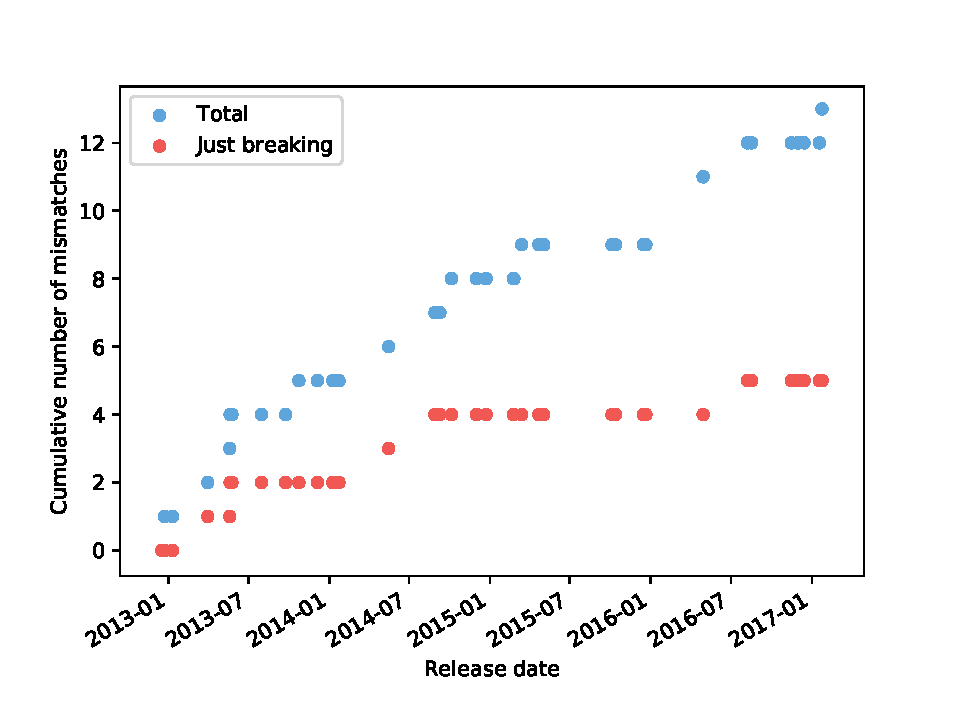
\includegraphics[height=0.4\textheight]
{images/evaluation/requests_cumulative_mismatches}
\caption{Cumulative mismatches over time (\textit{Requests})}
\label{RequestsCumulativeMismatches}
\end{figure}

\begin{figure}[]
\centering
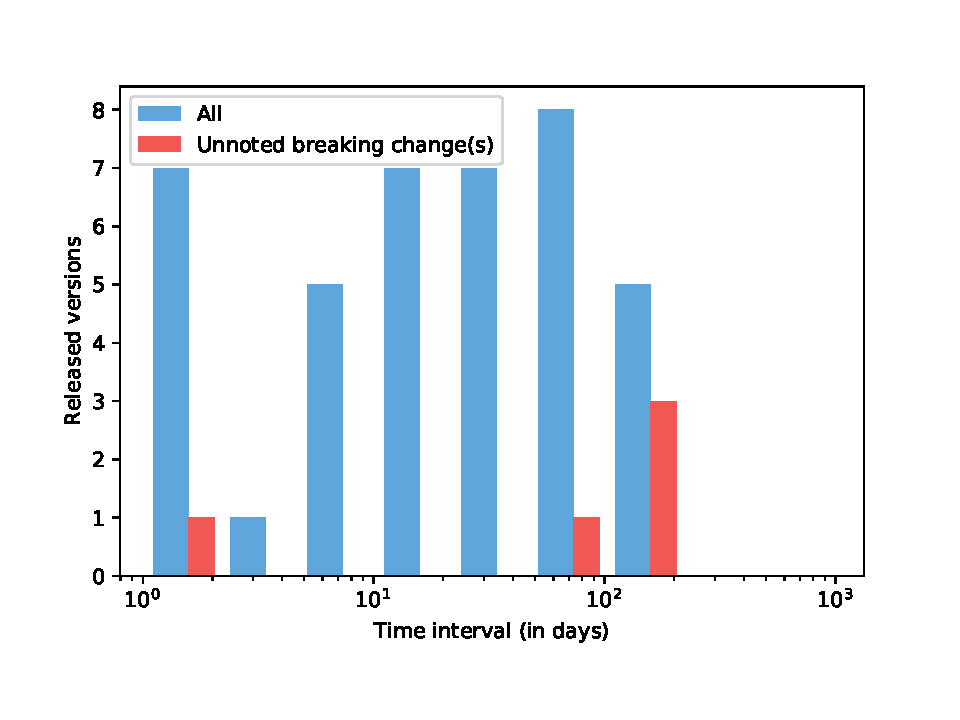
\includegraphics[height=0.4\textheight]
{images/evaluation/requests_introduced_changes}
\caption{Histogram of total versions vs. breaking mismatches in a time
interval (\textit{Requests})}
\label{RequestsHistogram}
\end{figure}

\subsubsection{Simplejson}

\textit{Simplejson} \cite{Simplejson} is a JSON parsing library which
has the highest number of downloads on PyPI across all projects. It is
also bundled with a standard CPython installation as part of the
standard library. Version \codeinline{3.0.0} is the lower bound for
evaluation as that is first one that supports Python 3. The upper
bound is \codeinline{3.10.0}, the latest one at the time of writing.

The reported number of mismatches with and without structural typing
is identical (tables \ref{SimplejsonNonStructural} and
\ref{SimplejsonStructural}). Evidently the method set used on a
parameter doesn't change significantly, and when it does change, it
happens to coincide with other changes that warrant the same version
bump. Given that only 39 versions were evaluated, it is not
unreasonable to say that the latter is possible.

\noindent
\begin{minipage}[t]{0.5\textwidth}
\begin{table}[H]
\centering
\begin{tabular}{|lr|}
All versions & 39 \\
Mismatches & 6 \\
Mismatches (breaking) & 1 \\
Proportion of mismatches & 15\% \\
Proportion of mismatches (breaking) & 2\%
\end{tabular}
\caption{\textit{Simplejson} statistics (w/o structural typing)}
\label{SimplejsonNonStructural}
\end{table}
\end{minipage}
\begin{minipage}[t]{0.5\textwidth}
\begin{table}[H]
\centering
\begin{tabular}{|lr|}
All versions & 39 \\
Mismatches & 6 \\
Mismatches (breaking) & 1 \\
Proportion of mismatches & 15\% \\
Proportion of mismatches (breaking) & 2\%
\end{tabular}
\caption{\textit{Simplejson} statistics (w/ structural typing)}
\label{SimplejsonStructural}
\end{table}
\end{minipage}

The sole unnoted breaking change is at the patch from
\codeinline{3.0.9} to \codeinline{3.1.0}. One exceptions and two
functions were moved from one module to another. That is noted in the
changelog, but evidently the authors did not consider it significant
enough to warrant a major version bump. Simplejson never officially
claims that it follows semantic versioning.

The remaining 5 mismatches are very similar to what was observed with
Requests. Very small additive changes to the API of some functions was
deemed a patch change, when Semver claims it should be a feature, and
improvements that don't impact the API bumped the minor version (which
is a valid interpretation).

Compared to Requests, the time between releases does not seem
to impact breaking changes (noted or unnoted) at all. Comparable
numbers of versions have been released at different intervals, but
only a single one resulted in an unidentified breaking change.
Moreover, that version was released only a few days after the previous
one (see fig. \ref{SimplejsonHistogram}).

\begin{figure}[H]
\centering
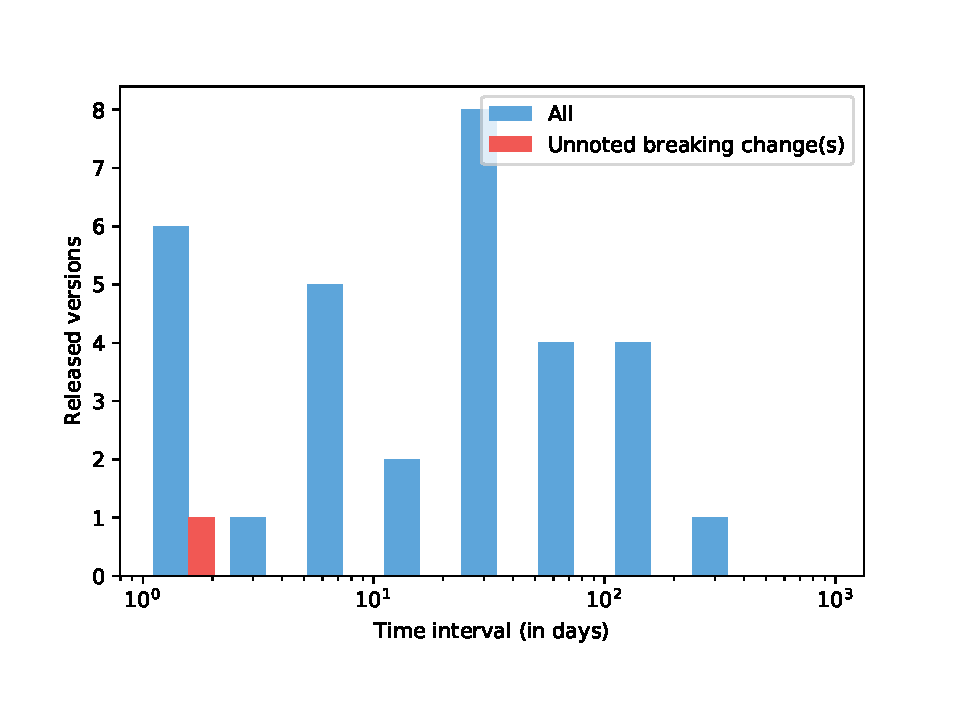
\includegraphics[height=0.32\textheight]
{images/evaluation/simplejson_introduced_changes}
\caption{Histogram of total versions vs. breaking mismatches in a time
interval (\textit{Simplejson})}
\label{SimplejsonHistogram}
\end{figure}

\subsubsection{Docopt}

\textit{Docopt} \cite{Docopt} is ``Pythonic argument parser'' for
creating command-line user interfaces. It is different from all other
evaluated projects because at the time of writing it does not yet have
a \codeinline{1.0.0} release. The API is not stable according to
Semver, so this project was mainly used to evaluate Autobump's
handling of projects with major version \codeinline{0}.

Only one mismatch is found when not using structural typing. A
function called \codeinline{parse_args} was renamed to
\codeinline{parse_argv} in version \codeinline{0.4.2}. Autobump
claimed that the version shoud have been \codeinline{0.5.0} because
that change was seen as breaking, but suppressed to only a minor bump
because the API is not yet stable.

\noindent
\begin{minipage}[t]{0.5\textwidth}
\begin{table}[H]
\centering
\begin{tabular}{|lr|}
All versions & 11 \\
Mismatches & 1 \\
Proportion of mismatches & 9\% \\
\end{tabular}
\caption{\textit{Docopt} statistics (w/o structural typing)}
\label{DocoptNonStructural}
\end{table}
\end{minipage}
\begin{minipage}[t]{0.5\textwidth}
\begin{table}[H]
\centering
\begin{tabular}{|lr|}
All versions & 11 \\
Mismatches & 2 \\
Proportion of mismatches & 18\% \\
\end{tabular}
\caption{\textit{Docopt} statistics (w/ structural typing)}
\label{DocoptStructural}
\end{table}
\end{minipage}

The one additional change found with structural typing enabled is
because of an additional method \codeinline{remove} being called on a
parameter. The surrounding usage implies that the argument is a list
and it is reasonable to expect that it would provide a
\codeinline{remove} method. Similarly to some cases in
Requests, Autobump is being overzealous.

\subsubsection{Hashids}

\textit{Hashids} \cite{Hashids} is a very small (one class with four
methods) library for generating unique string identifiers from
integers. It is a fairly recent projects, so all 10 released versions
support Python 3 and were evaluated. 4 out of them have major version
\codeinline{0} similarly to Docopt, whereas the 5\textsuperscript{th}
one is \codeinline{1.0.0}. This is useful to check whether Autobump
handles the boundary between unstable and stable API sensibly.

Similarly to Simplejson there is no difference in the
mismatches with structural typing enabled and disabled.

\noindent
\begin{minipage}[t]{0.5\textwidth}
\begin{table}[H]
\centering
\begin{tabular}{|lr|}
All versions & 10 \\
Mismatches & 4 \\
Mismatches (breaking) & 1 \\
Proportion of mismatches & 40\% \\
Proportion of mismatches (breaking) & 10\% \\
\end{tabular}
\caption{\textit{Hashids} statistics (w/o structural typing)}
\label{HashidsNonStructural}
\end{table}
\end{minipage}
\begin{minipage}[t]{0.5\textwidth}
\begin{table}[H]
\centering
\begin{tabular}{|lr|}
All versions & 10 \\
Mismatches & 4 \\
Mismatches (breaking) & 1 \\
Proportion of mismatches & 40\% \\
Proportion of mismatches (breaking) & 10\% \\
\end{tabular}
\caption{\textit{Hashids} statistics (w/ structural typing)}
\label{HashidsStructural}
\end{table}
\end{minipage}

One of the mismatches stems from a simple mistake -- a version was
omitted. In the release history \codeinline{0.8.3} follows
\codeinline{0.8.1}. Autobump correctly suggests that
\codeinline{0.8.2} should have been the appropriate number.

Version \codeinline{0.8.4} is the last version with an unstable API,
the following one being \codeinline{1.0.0}. At that point Autobump
suggests that it should have been \codeinline{0.9.0}, reluctant to
bump the major version making the API official. This is valid
behaviour and this is definitely a case when Autobump's suggestion can
be discarded because it is up to the authors to decide when to publish
an API.

The other non-breaking mismatch comes from a performance optimization
done in \codeinline{1.2.0} where Autobump suggests it should have been
\codeinline{1.1.1}, a patch change. This is an identical situation to
ones found in the previous libraries.

The only unnoted breaking change is renaming the methods
\codeinline{encrypt} and \codeinline{decrypt} to \codeinline{encode}
and \codeinline{decode} respectively. Those methods provide the core
functionality of the library, yet the authors deemed that (rather
dangerously) a patch change.

\subsection{Java}

\begin{table}[H]
\centering
\caption{Java projects chosen for evaluation}
\label{JavaProjectsForEvaluation}
\begin{tabular}{|l|l|l|p{10cm}|}
\hline
\textbf{Project} & \textbf{Size} & \textbf{Dependants}
& \textbf{Semantically versioned} \\
\hline
\codeinline{guava} & 150 000 LOC & 10700 & A contributor remarks ``we
actually do use semantic versioning with
Guava''\footnote{https://github.com/google/guava/issues/1682}. \\
\codeinline{mockito} & 11000 LOC & 8415 & \codeinline{CONTRIBUTING}
claims that ``semantic versioning is rigorously maintained'', but is
then implied that this applies only for after major version
\codeinline{2}. \\
\codeinline{gson} & 8000 LOC & 3400 & Seems like it, not officially. \\
\hline
\end{tabular}
\end{table}

Evaluation of Java projects using the native handler proved to be difficult.
Two out the three selected projects happened to have quite a long
history during which they have changed their build system several
times. This makes it impossible to specify a single build command and
evaluate the entire repository in one run. Instead, evaluations had to
be done one range at a time, and then the results merged together.

Furthermore, early versions of some projects (most notably Guava)
require ancient versions of Java. Given the impracticality of
maintaining several versions of the JDK, along with respective
versions of build systems and so on, those versions were just skipped
when using the native handler.

A final hurdle was that compiling complex Java projects like these
ones is slow -- when running the \codeinline{java_native} handler it
was noticeably an order of magnitude slower than \codeinline{java_ast}.

\subsubsection{Guava}

\begin{wraptable}{r}{0.45\textwidth}
\centering
\caption{\textit{Guava} statistics (using AST handler)}
\label{GuavaStatistics}
\begin{tabular}{|lr|}
All versions & 28 \\
Mismatches & 6 \\
Mismatches (breaking) & 3 \\
Proportion of mismatches & 21\% \\
Proportion of mismatches (breaking) & 10\% \\
\end{tabular}
\end{wraptable}

\textit{Guava} \cite{Guava} is a set of core libraries that extend the
Java standard library. It is one of the most widely used Java
projects.

The \codeinline{java_native} handler was not of much use; the version
ranges \textit{2 -- 6} and \textit{10 -- 18} did not compile. Although
out of the 5 versions that did compile, there weren't any mismatches.

One mismatch in version \textit{11.0.1} sees two utility methods
removed, but they were marked as deprecated beforehand. Semver is
ambiguous as to whether deprecated methods are part of the public API,
so this is not necessarily a breaking change.

The remaining 4 are clear deviations from Semver. Version
\textit{2.0.0} introduces many new features compared to
\textit{1.0.0}, but no breaking changes. The same applies for versions
\textit{5.0.0} and \textit{6.0.0}. In version \textit{10.0.1} some
deeply nested utility methods were removed, which were nevertheless
part of the public API.

\subsubsection{Mockito}

\textit{Mockito} \cite{Mockito} is a mocking library. It is one of few
libraries that outright claim to follow Semver, although that only
applies since version \textit{2.0.0} \cite{MockitoSemver}.

\begin{wraptable}{r}{0.45\textwidth}
\centering
\caption{\textit{mockito} statistics (using AST handler)}
\label{MockitoStatistics}
\begin{tabular}{|lr|}
All versions & 220 \\
Mismatches & 76 \\
Mismatches (breaking) & 44 \\
Proportion of mismatches & 33\% \\
Proportion of mismatches (breaking) & 20\% \\
\end{tabular}
\end{wraptable}

Although Semver is followed officially after \textit{2.0.0}, there is
no difference between the rate of mismatches before and after this
version (fig. \ref{MockitoCumulativeMismatches}).

Breaking mismatches are mostly due to the same reasons as with other
libraries -- removing little-used methods or classes, and making small
backwards-compatible changes to the API without bumping the minor
version number. These happen frequently both before and after Mockito
started to follow semantic versioning.


Evaluation using the native handler was hugely problematic and did not
yield any results. Mockito at several points changes the build system
configuration (and sometimes the build system itself), making it
impossible to have a single compile command and build root pair. For
this reason, the history of the project was manually probed to find
where those changes are and perform an evaluation for every change.
The results were then going to be merged together.

\begin{figure}[H]
\centering
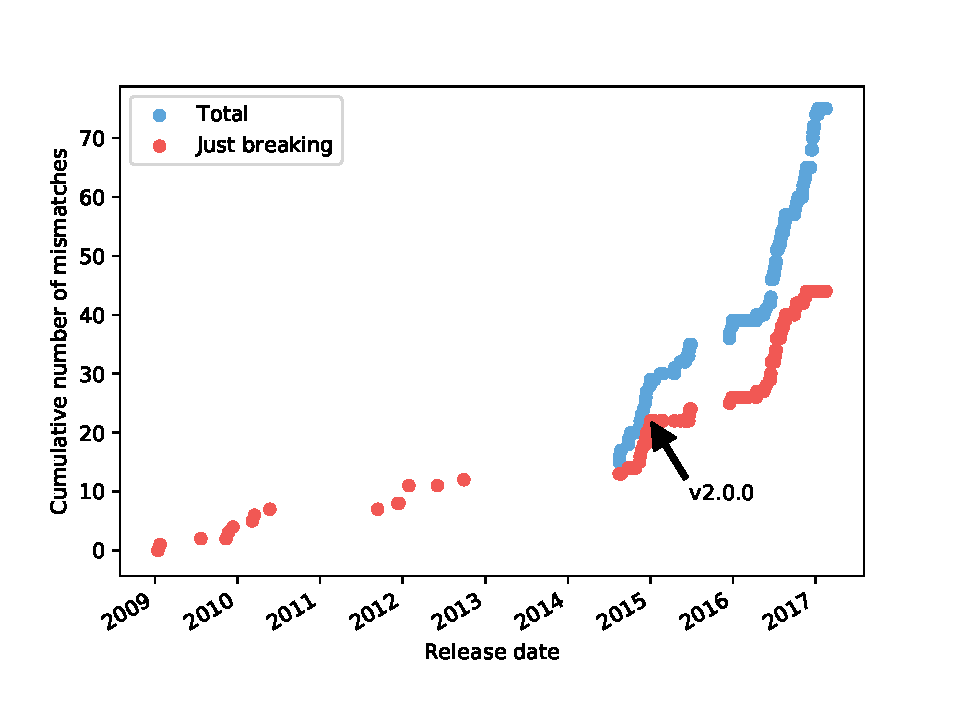
\includegraphics[height=0.4\textheight]
{images/evaluation/mockito_cumulative_mismatches}
\caption{Cumulative mismatches over time (\textit{mockito})}
\label{MockitoCumulativeMismatches}
\end{figure}

However, these changes turned out to be more frequent than expected.
Even when the correct build system was invoked with the correct
parameters, builds still often times failed with non-descriptive error
messages like \codeinline{NullPointerException}. Moreover, there was
no consistent way to skip running the test suite. Later versions of
Mockito are built using Gradle, and the the standard
approach of passing \codeinline{-x test} to ignore the task
\codeinline{test} did not work half the time based on some combination
of the version of Gradle and the configuration.

\subsubsection{GSON}

\textit{GSON} \cite{GSON} is serialization and deserialization library that
can convert Java objects to JSON and vice versa.

\noindent
\begin{minipage}[t]{0.5\textwidth}
\begin{table}[H]
\centering
\begin{tabular}{|lr|}
All versions & 30 \\
Dropped versions & 0 \\
Mismatches & 12 \\
Mismatches (breaking) & 10 \\
Proportion of mismatches & 40\% \\
Proportion of mismatches (breaking) & 33\% \\
\end{tabular}
\caption{\textit{GSON} statistics (using AST handler)}
\label{GSONASTStatistics}
\end{table}
\end{minipage}
\begin{minipage}[t]{0.5\textwidth}
\begin{table}[H]
\centering
\begin{tabular}{|lr|}
All versions & 30 \\
Dropped versions & 2 \\
Mismatches & 13 \\
Mismatches (breaking) & 12 \\
Proportion of mismatches & 46\% \\
Proportion of mismatches (breaking) & 42\% \\
\end{tabular}
\caption{\textit{GSON} statistics (using native handler)}
\label{GSONNativeStatistics}
\end{table}
\end{minipage}

While the proportions of mismatches for GSON are slightly higher than
other projects, there are no new unique reasons for them -- the most
frequent cause of a breaking mismatch is the removal of an unimportant
method or class. Those changes just happen more often.

\subsection{Clojure}

\begin{table}[H]
\centering
\caption{Clojure projects chosen for evaluation}
\label{ClojureProjectsForEvaluation}
\begin{tabular}{|l|l|l|p{10cm}|}
\hline
\textbf{Project} & \textbf{Size} & \textbf{Dependants}
& \textbf{Semantically versioned} \\
\hline
\codeinline{cheshire} & 1200 LOC & 961 & Seems like it, not
officially. \\
\codeinline{nippy} & 2200 LOC & 105 & Seems like it, not officially. \\
\codeinline{core.typed} & 43 000 LOC & 49 & Seems like it, not
officially. \\
\hline
% \\
\end{tabular}
\end{table}

\subsubsection{Cheshire}

\textit{Cheshire} \cite{Cheshire} is a ``fast JSON encoder and
decoder''. It is a relatively mature Clojure project, being at major
version \codeinline{5} at the time of writing and being one of the
most popular Clojure libraries. Although type hinting is optional, it
is used for almost every function in the library.

The very first pair of versions was ignored during evaluation, because
the first version \codeinline{1.1.0} has misconfigured paths and the
namespaces it defines are inaccessible, not even when working from a
manually created REPL.

There seems to be a clear indication that the project has stabilised
over time (fig. \ref{CheshireCumulativeMismatches}), seeing frequent,
unnoted in the version number, breaking changes for the first 2 years
of development, and then not for the next 4 years. It's noteworthy
that this stabilisation happened only at major version \codeinline{5}
and that the frequency of releases has gone down since then. There
were 3.96 releases per 100 days in that 2-year interval, compared to
only 1.70 for the entirety of the project's history.

\begin{table}[H]
\centering
\caption{\textit{Cheshire} statistics}
\label{CheshireStats}
\begin{tabular}{|lr|}
All versions & 38 \\
Dropped versions & 1 \\
Mismatches & 19 \\
Mismatches (breaking) & 7 \\
Proportion of mismatches & 51\% \\
Proportion of mismatches (breaking) & 18\% \\
\end{tabular}
\end{table}

Breaking mismatches are evenly divided between two causes:

\begin{enumerate}[(i)]
\item Refactoring one function into several other, similarly-named
functions. All of these changes bump the minor version number, even
though the original function is removed. For example, version
\codeinline{2.1.0} refactors \clojureinline{factory} into
\clojureinline{make-json-factory} and
\clojureinline{make-smile-factory}.
\item Introducing type hints where there were previously none, or
changing them to an incompatible type.
\end{enumerate}

This project also shows a large number of non-breaking mismatches,
accounting for about 30\%. The vast majority of those are because of
one or two small (public) functions being introduced and only bumping
the patch version number. Only two (\codeinline{5.7.0} and
\codeinline{5.5.1}) are because of making legitimate improvements that
don't impact the API.

\begin{figure}[H]
\centering
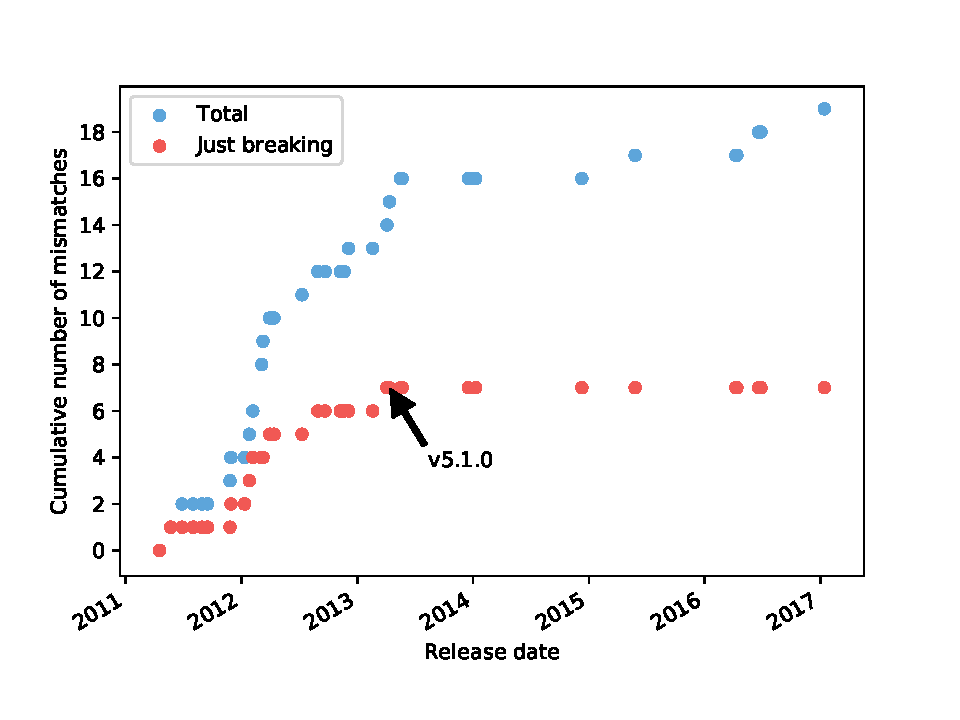
\includegraphics[height=0.4\textheight]
{images/evaluation/cheshire_cumulative_mismatches}
\caption{Cumulative mismatches over time (\textit{Cheshire})}
\label{CheshireCumulativeMismatches}
\end{figure}

\subsubsection{Nippy}

\textit{Nippy} \cite{Nippy} is a ``high-performance serialization
library''. It has 70 tagged releases, but nearly half of them carry a
label after the version number. For example version
\codeinline{v2.5.0} has 6 variants -- the final one, two release
candidates and three betas. Only the actual final version is compared
to its successor in evaluation, which brings down the number of
releases to 32.

\begin{wraptable}{r}{0.45\textwidth}
\centering
\caption{\textit{Nippy} statistics}
\label{NippyStats}
\begin{tabular}{|lr|}
All versions & 32 \\
Mismatches & 14 \\
Mismatches (breaking) & 6 \\
Proportion of mismatches & 43\% \\
Proportion of mismatches (breaking) & 18\% \\
\end{tabular}
\end{wraptable}

Nippy shows a trend of stabilisation similar to
Cheshire (fig. \ref{NippyCumulativeMismatches}). For a period
of about 2 years between versions \codeinline{1.2.0} and
\codeinline{2.7.0} there is a large number unnoted breaking changes,
which then plateaus. The frequency of releases in that interval is
also larger than the one for the entirety of the project: 5.60 per 100
days, compared to only 3.74 per 100 days.

\begin{figure}[]
\centering
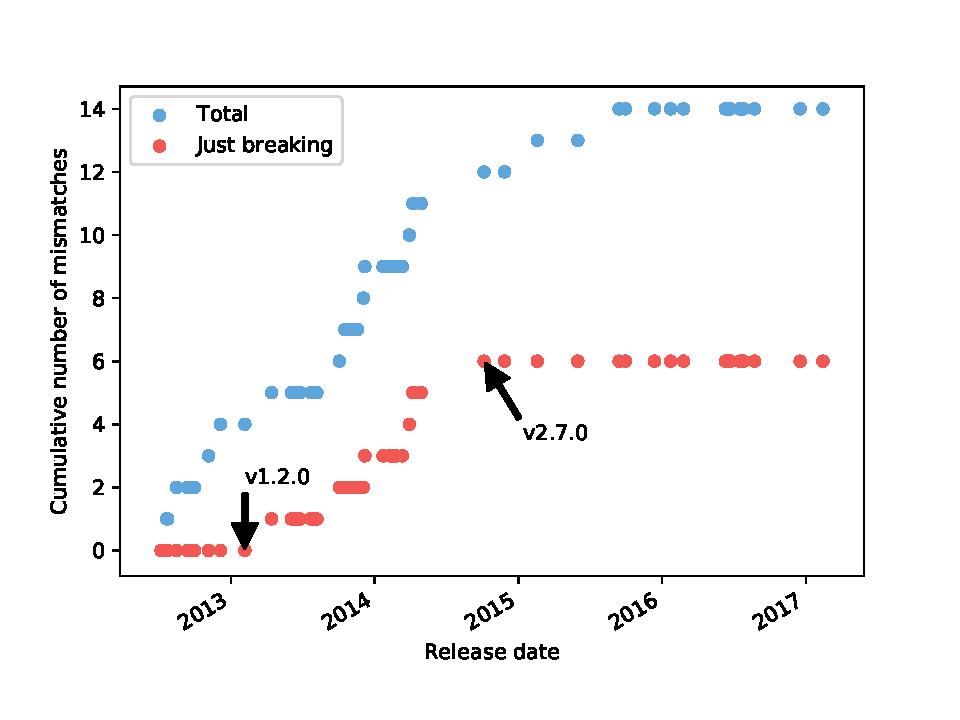
\includegraphics[height=0.4\textheight]
{images/evaluation/nippy_cumulative_mismatches}
\caption{Cumulative mismatches over time (\textit{Nippy})}
\label{NippyCumulativeMismatches}
\end{figure}

All 6 breaking mismatches see at most 2 entities being removed or
renamed. In one case renaming happens not because of refactoring, but
because of a typo: \codeinline{2.6.1} corrects the function
\clojureinline{freezeable?} to \clojureinline{freezable?} which was
introduced in the previous version \codeinline{2.6.0}. Fixing a typo
was considered a patch-level change by the authors, even though that
typo was at that point part of the public API.

The distribution and reasoning behind non-breaking mismatches is
nearly identical to what was observed in \textit{cheshire} -- nearly
all such changes are because of a small number of public functions
being introduced and not bumping the minor version number.

\subsubsection{Core.Typed}

\textit{Core.Typed} \cite{CoreTyped} is the library that provides
optional static typing for Clojure. It is part of Clojure 1.8 and
future versions. Given that this is a relatively recent addition to
Clojure, there are not many projects that use it consistently or have
been using it long enough to warrant evaluation -- so the library
itself was chosen for evaluation.

\begin{wraptable}{r}{0.45\textwidth}
\centering
\caption{\textit{Core.Typed} statistics}
\label{CoreTypedStats}
\begin{tabular}{|lr|}
All versions & 144 \\
Mismatches & 142 \\
Proportion of mismatches & 98\% \\
\end{tabular}
\end{wraptable}

Unfortunately Core.Typed does not have a stable API, the highest
version reached so far being \textit{0.3.9}. Every single release has
breaking changes, and Autobump's behaviour of bumping the minor
version instead of the major whenever there's a breaking change before
\textit{1.0.0} leads to a huge number of mismatches.

Another way to handle breaking changes before \textit{1.0.0} is to
simply ignore them and only consider the other two categories Autobump
detects. However, it would not have a significant difference for this
project -- the library has always been in rapid development and nearly
every patch release includes at least one new function.

\subsection{Summary}

Several observations about the projects themselves and Autobump can be
made from the first round data:

\begin{enumerate}[(i)]
\item Projects that officially claim to follow semantic versioning
don't appear to do any better than projects that don't.
\item The proportions of mismatches are comparable across the different
languages, and it does not seem that language-specific features impact
them.
\item The most frequent causes for mismatches are very similar for the
different languages. Even if a project claims to follow semantic
versioning, some version bumps are still done according to a
subjectively determined relative importance of the change, rather than
what the scheme actually demands.
\item The impact of most unnoted changes is likely not hugely
significant for the majority of users, but has the potential to be.
\item The length of time passed since the previous release of a
project may be proportional to the likelihood of the new release
introducing an unnoted breaking change.
\item \textit{Some} projects have demonstrated a trend of stabilising
over time, i.e. better following semantic versioning in later stages
of development.
\item Using a common representation for all languages does not seem to
handicap the ability to detect API changes for any particular
language.
\item Structural typing may be an unnecessary or even harmful feature:
for some projects, like Requests, the proportion of mismatches doubles
when enabled.
\item The assumption made by \codeinline{java_native} that one build
command can be used to build a project at all revisions is
unrealistic, as 2 out of the 3 Java projects have shown. It may be a
good idea to consider an approach where Autobump is invoked by the
build system at appropriate times, rather than the other way around.
\end{enumerate}

Overall, the data suggests that these projects would have slightly
benefited from using a tool such as Autobump to prevent subjectivity
from influencing versioning decisions.

\section{Automated evaluation}

In addition to the previous round, a large scale evaluation was
attempted on 632 Python projects. It was almost completely automated,
with scripts responsible for each step -- from suggesting projects, to
gathering metrics.

\subsection{Methodology}

The number 632 is not arbitrary. To gather Python projects with
varying popularity, the websites \textit{http://pypi-ranking.info} and
\textit{http://pypi.org} were scraped. The first one was used to get a
listing of all published projects in decreasing order of popularity
and check for Python 3 compatibility, and the second one was used to
visit the official page of each project and search via a regular
expression for a GitHub\footnote{Earlier iterations of the scraper
script tried to use a more general regular expression, but that proved
to be very erroneous, so it was limited to the most popular hosting
for repositories.} repository. As projects get less popular, their
support for Python 3 decreases rapidly, as they have not seen a
release in some time. After reaching zero (number of downloads) the
ones that support it get extremely sparse, so the scraping was cut off
soon after that point. That is not to say that there are only 632
Python projects that support Python 3 and have a download count larger
than zero -- these are only the ones for which a GitHub link was found
reliably on the module's PyPI page.

Note that not all of these projects are guaranteed to be libraries;
there is no good way to filter out end user applications. Instead, we
just assume the modules the project defines can be imported and used
by other applications (this is technically true for all Python
projects). Although Autobump itself is an end-user application and not
a library, it still adheres to Python naming conventions to
distinguish public from private code. If all projects do the same then
there will be no difference whether they are applications or
libraries.

After the list of repositories was obtained, each one was cloned in a
separate directory. Of 632 repositories,
605 were cloned successfully, the rest failing because they were
private or removed.

A generic configuration file was constructed
that ignores frequently encountered directories and files such as
\codeinline{tests} and \codeinline{setup.py}. After that, all projects
were evaluated from their very first release to the very last, all
using the same configuration file.

Just like the manual evaluation of Python projects, the automated was
done twice -- with and without structural typing.

\subsubsection{Limitations}

Not having a project-specific configuration files and using a generic
one for all projects is not ideal. It was fully expected that this
would introduce some noise in the final data.

There is an obvious problem with Python 3 compatibility -- although
PyPI can rightfully claim that a project supports Python 3 and it ends
up in this list of 632 repositories, it is not guaranteed that all
versions support Python 3. There is no good automatic way of
determining the first version that does so. Initially, a heuristic was
used. When the Python handler encounters a file it cannot parse, it
either warns the user or outright fails with an error depending on how
it is configured. The generic configuration file directs Autobump to
steamroll through the entire projects only warning about unparseable
files. Unparseable files most likely indicate Python 2 code, so the
first version that doesn't raise such a warning is taken to be the
first version as far as evaluation is concerned.

However, this approach led to too many versions, sometimes entire
projects, being dropped. It is not uncommon for projects to have both
Python 2 and Python 3 code in their repository. Instead, while
unparseable files are still omitted, Autobump still considers others.
This potentially leads to introducing false negatives, but the impact
of that on the final data ought to be smaller than dropping too many
versions -- library code written in Python 2 is frequently compatible
with 3 without any modifications. User-facing parts of the projects
using \pythoninline{print} statements without parantheses are more
likely to fail. Nevertheless, when examining the final results it
should be taken into account that they are expected to be slightly
skewed towards a lower number of mismatches because of source files
being ignored.

\subsection{Results}

Out of the 605 successfully cloned projects, only 403 were
successfully evaluated. The remaining were discounted because they had
less than 2 released versions\footnote{This means less than 2 tags in
the repository. It is entirely possible that the project has releases
which are not tagged, but the script can't find that out.}, so no
adjacent pairs of versions could be compared.

Prior to any evaluation, it was noted that nearly all projects have
less than 50 releases, with the majority having less than 10 (fig.
\ref{DistributionAllVersions}). Morevoer, looking at the largest major
version that projects have seen it was found that there was a
disproportionate number of projects that have never seen a
\textit{1.0.0} release (fig. \ref{DistributionLargestMajor}).

Having this information in mind, three data sets were constructed to
avoid skewing the statistical results because of outliers: one
comprising all 403 projects, a second one containing only projects
which reach version \textit{1.0.0} and a third one with projects that
have at least 10 released versions. Note that some projects can fall
in more than one category (fig. \ref{Datasets}). A fourth data set was
considered, containing projects that had a higher degree of
popularity, but ultimately not used because its contents heavily
coincided with the one containing projects that have reached version
\textit{1.0.0}.

\subsubsection{Without structural typing}

After generating statistics about the numbers of total and breaking
mismatches in the different data sets (fig. \ref{BoxplotsMismatches}
and \ref{BoxplotsBreaking}), several observations were made. The
median percentage of total mismatches in projects with a published API
(50\%) is only slightly higher than the median for projects with at
least 10 releases (47\%), which is in turn only slightly higher than
the median for all projects (44\%). Not only the median, but indeed
the whole distribution of the percentage of mismatches steadily shifts
downwards, which is more evident in figures
\ref{DistributionPublishedAPI}, \ref{DistributionTenReleases} and
\ref{DistributionAllProjects}.

Moreover, looking at the median percentages of breaking mismatches
(0\%, 12\% and 0\% respectively) it is clear that non-breaking
mismatches are much more frequent than breaking. During the manual
evaluation phase it was found that they mostly stem from making small
backwards-compatible changes without bumping the minor version number,
and from bumping the minor version when making improvements that don't
affect the API. Given that the proportion of breaking versus
non-breaking mismatches here is similar, it is possible that the
reasons are also similar.

The 0\% median breaking mismatches in two of the data sets is
unsurprising, given that only 172 of the 403 projects have ever
reached major vesion 1 and Autobump by design never bumps a project at
major version 0 to 1. Separating the ones that have reached
\textit{1.0.0} (or higher) in another data set is more representative
of how Autobump behaves with projects that have a longer history.

The 12\% median number of breaking mismatches is only slightly higher
than what was found during the manual evaluation of Python projects
with structural typing disabled -- 10\%\footnote{Considering only the
three projects that have reached major version 1, i.e.
discounting Docopt.}.

Across all projects, there is no clear indication that the length of
time passed between two adjacent releases has bearing on whether a
breaking change went unnoted (fig. \ref{HistogramAllProjects}). The
highest observed ratio of breaking mismatches to all released versions
is around the 100-day mark, but it does not dominate the other time
intervals.

Additionally, out of the 172 projects that have a stable API, 164 were
found to have at least one release before major version 1. The ratio
$\frac{\text{mismatches before first major release}}{\text{mismatches
after first major release}}$ for projects that have at least one
mismatch from before the first release with a stable API
\footnote{Projects with no mismatches before the first release most
likely indicate that those versions don't support Python 3 and are
skewing the data.} was found to be in the range $(0, 1]$ (fig.
\ref{StableBoundaryRatio}) for the majority of projects -- indicating
that major version 1 is indeed considered (at least partly) to publish
an API.

\begin{figure}[H]
\centering
\caption{Histogram of ratios $\frac{\text{mismatches before first
major release}}{\text{mismatches after first major release}}$}
\label{StableBoundaryRatio}
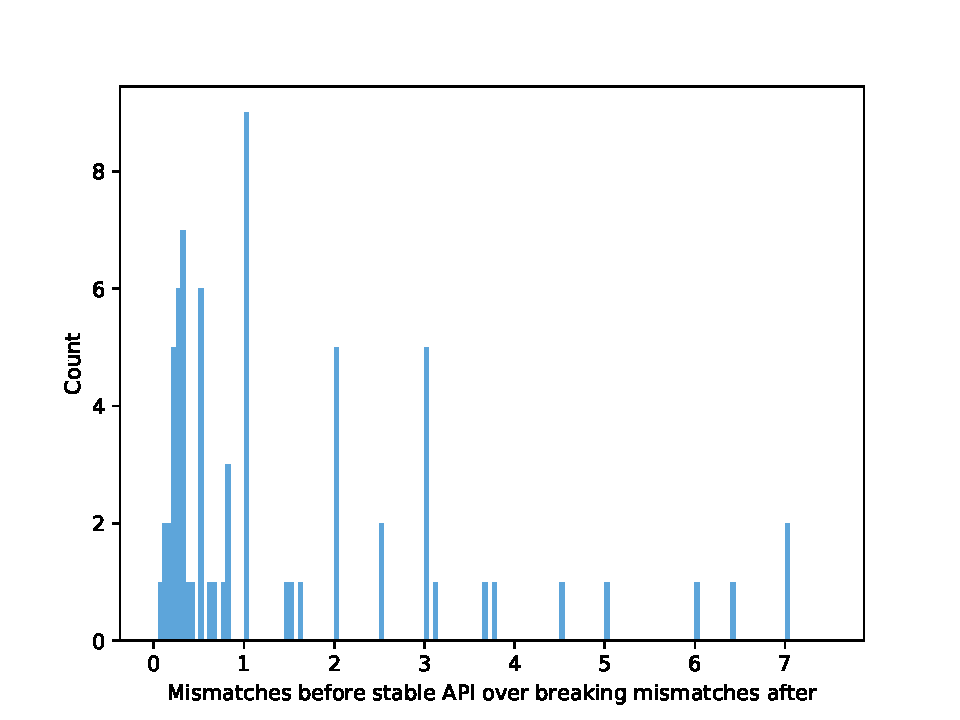
\includegraphics[height=0.3\textheight]{images/evaluation/ls_stable_boundary}
\end{figure}

\subsubsection{With structural typing}

With structural typing enabled, somewhat suprisingly, there is a very
small upward shift in the number of breaking mismatches (fig.
\ref{StrBoxplotsMismatches} and \ref{StrBoxplotsBreaking}). All data
sets seem to equally affected. This is contrary to what was observed
in the first round, where for some projects structural typing almost
doubled the number of breaking mismatches.

The proportions of breaking mismatches to all released versions in
different time intervals are uniformly slightly higher (fig.
\ref{StrHistogramAllProjects}).

\subsubsection{Summary}

Overall, the results from the second round of evaluation show that the
projects selected in the first round were indeed
representative\footnote{As far as adherence to semantic versioning is
concerned.} of the Python ecosystem as a whole. The notable exception
is that structural typing actually has a much smaller impact than what
the first round would suggest.

Some projects, like Requests, suggested that the number of unnoted
breaking changes may be proportional to the time interval that has
elapsed since the last release. However, data gathered from a larger
sample size shows that this is not the case.

\chapter{Conclusion}
\label{Conclusion}

\section{Summary}

The goal of this project was to develop and evaluate Autobump -- a
tool that can automatically propose the next semantic version of
projects in different languages based on changes to the public API.
For this task, a common API representation was constructed and two
different approaches were considered for converting to it -- parsing
the AST and introspection -- and both were implemented where suitable.

The tool was demonstrated to work reasonably well through acceptance
testing and evaluation against real-world libraries. Two rounds of
evaluation found that semantic versioning is indeed not adhered to
strictly in all considered languages, even by projects that claim to
do so. It was also shown that had they employed a tool such as
Autobump, their adherence would have been higher.

The final\footnote{Meaning the latest version as of the date of
submission of this dissertation.} version of Autobump is not a
prototype, but is still beta-quality software that may not be suited
to production use. It is, however, almost fully functional and usable.

\section{Future work}

\subsection{Changelog generation}

The common API representation has not lended itself nicely to
generating sensible changelogs. CAPIR abstracts away language-specific
terminology, which does not impact version assignment, but it does
lead to less intelligible changelogs. One of the worst examples, as
seen in the Mockito library, is how replacing the signature of a
method with another one is logged:

\begin{center}
\begin{BVerbatim}
org.mockito.Mockito.mock: Function was overloaded
org.mockito.Mockito.mock: Overloaded function removed
\end{BVerbatim}
\end{center}

Although logs like these do shed light on the versioning decisions
that Autobump makes, they may not always be useful for direct
consumption by users. One possible solution to this problem would
be to have the language handlers provide appropriate labels for CAPIR
change patterns, although that would complicate the current implementation's
architecture.

An alternative is to even further decentralise and reduce Autobump to
a very small core or even just a standard which can then be
implemented in the target languages. However, in doing that the point
of having a single tool and a common API representation is somewhat
lost. This way of doing things is arguably worse than both the current
implementation and having standalone, unrelated tools. Given that
changelog generation is the only major problem area as the final
version of Autobump stands, there is little benefit to pursuing this
approach.

\tricksubsection{Language handler for binary files}

It is possible to build a language handler that does not work with a
specific language, but rather a specific binary file format. This, in
effect, monitors changes to the ABI.

The ABI could be determined only if the binary file contains debugging
information in a known format, such as DWARF \cite{Dwarf}. The handler
would require a build command, similarly to the
\codeinline{java_native} handler, which generates binary files
containing debugging information.

An extension like that would be of benefit when clients are provided
binary files directly and expected to link to that. It is also
language-agnostic, with a handler that reads DWARF being able to work
with C, C++, Rust and others that allow for C interoperability.

\tricksubsection{Integration with development tools}

The natural continuation of Autobump's development would be to
integrate with other development tools, mostly continuous integration
systems. Integrating with plugins such as \textit{Release}
\cite{JenkinsRelease} for Jenkins would allow for automated and frequent
deployments with the correct semantic version.

Another possibility, albeit less useful, would be developing a plugin
for integrated development environments, so that changes to the API
determined by Autobump can be immediately highlighted for the
developer and visited.

\tricksubsection{A better automated versioning scheme}

Semantic versioning is designed to be suitable for both humans and
machines. As noted by Jeremy Ashkenas \cite{WhySemanticVersioningIsnt}
it tries to compress too much information into just a few numbers.
This is presumably done so that it remains intelligible to human
readers. Because the automated suggestion of the next semantic version
by code inspection was found to be viable by this project and others,
it may be worthwhile to consider a new versioning scheme that contains
additional information found by looking at the code. One extension to
semantic versioning that would be immediately useful is:

\begin{center}
$\mathrm{Major.Minor.Patch}:\mathrm{Difference}$ \\
where $\mathrm{Difference}$ is the tree edit distance between this
version's AST and the previous one's
\end{center}

Consider having two sequential patch releases: \textit{1.0.2:120} and
\textit{1.0.3:1}. Because of the large AST edit distance between
\textit{1.0.2:120} and the previous version, it is likely that this
version fixes one or more major bugs. Similarly, it can be said that
if the version were \textit{1.1.0:120}, it is likely to contain
significant performance improvements or a larger number of new
features. In contrast, \textit{1.0.3:1} is most definitely a minor
correction. If an automated package manager was making decisions about
upgrading dependencies, it may decide to withhold upgrading on
relatively unimportant releases like \textit{1.0.3:1} in some
situations.

There is a myriad of possibilities about what sort of additional
information can be encoded into the version number. Having a
versioning scheme that is better suited to automation could
potentially avoid the problems with Semver as shown in this
dissertation -- little formal adoption and somewhat poor adherence.

%=== Appendices ===

\begin{appendices}

\chapter{Running Autobump in practice}
\label{AutobumpInPractice}

Autobump requires at least Python 3.5. The easiest way to run it is to
install the published version from PyPI by running \codeinline{pip
install autobump}. This is going to pull in all necessary dependencies
and check whether the version of Python is appropriate. Autobump
should then be available under the executable in \codeinline{PATH}
named \codeinline{autobump}.

Alternatively, Autobump can be used from within a virtual environment
that has all dependencies preinstalled (see
\codeinline{requirements.txt}) by setting the \codeinline{PYTHONPATH}
environment variable appropriately. An executable won't be available
because \codeinline{setuptools} takes care of creating it when making
the distribution package, but Autobump can be called as a module by
running \codeinline{python -m autobump}. This approach is not recommended.

\section{Rundown of options}
\label{RundownOptions}

\begin{itemize}
\item \codeinline{-h}: prints usage information
\item \codeinline{--changelog CHANGELOG}: generates a changelog in the
file \codeinline{CHANGELOG}
\item \codeinline{--changelog-stdout}: prints a changelog to standard
out
\item \codeinline{--debug}: prints debugging information to standard
error (implies \codeinline{--information})
\item \codeinline{--information}: print progress information to
standard error
\item \codeinline{--silence}: silence all output except for fatal
errors and final results
\item \codeinline{--repo REPO}: location of repository, defaults to current
directory
\item \codeinline{--from IDENTIFIER}: identifier of earlier revision,
defaults to last tag
\item \codeinline{--to IDENTIFIER}: identifier of later revision, defaults to
last commit
\item \codeinline{--from-version FROM_VERSION}: considers the earlier
revision to be version \codeinline{FROM_VERSION}, attempts to guess
from identifier name if not specified
\item \codeinline{--build-command BUILD_COMMAND}: executes
\codeinline{BUILD_COMMAND} as a shell command in the root of the
project in order to build it
\item \codeinline{--build-root BUILD_ROOT}: location relative to
project root where generated artefacts get placed after building
\item \codeinline{--evaluate}: run in evaluation mode
\item \codeinline{--export-config}: print current configuration
\end{itemize}

\section{Rundown of configurables}
\label{RundownConfigurables}

Configurable options are grouped into categories.

\begin{itemize}
\item \codeinline{autobump}
\begin{itemize}
\item \codeinline{git}: path to Git executable
\item \codeinline{hg}: path to Mercurial executable
\item \codeinline{clojure}: path to Clojure executable
\item \codeinline{java}: path to Java class runner
\item \codeinline{javac}: path to Java compiler
\end{itemize}
\item \codeinline{ignore}
\begin{itemize}
\item \codeinline{files}
\item \codeinline{dirs}
\item \codeinline{entities}
\end{itemize}
\item \codeinline{only_consider}
\begin{itemize}
\item \codeinline{files}
\item \codeinline{dirs}
\item \codeinline{entities}
\end{itemize}
\item \codeinline{python}
\begin{itemize}
\item \codeinline{omit_on_error}: skip a Python source file that
can't be parsed
\item \codeinline{structural_typing}: determine type of parameters by
looking at their usage
\item \codeinline{type_hinting}: consider type hints
\end{itemize}
\item \codeinline{java_native}
\begin{itemize}
\item \codeinline{classpath}
\end{itemize}
\item \codeinline{java_ast}
\begin{itemize}
\item \codeinline{omit_on_error}: skip a Java source file that can't
be parsed
\item \codeinline{error_on_external_types}: immediately give if the
AST of a class is not available
\end{itemize}
\item \codeinline{clojure}
\begin{itemize}
\item \codeinline{classpath}
\item \codeinline{omit_on_error}: skip a Clojure source file that
can't be parsed
\end{itemize}
\end{itemize}

\section{Task management}

Autobump's source code comes with a regular \textit{GNU Make} Makefile
that is used for task management. The different targets are:

\begin{itemize}
\item \codeinline{lint}: runs a linter against all source code (except
for tests) and fails the target if there are formatting issues
\item \codeinline{unit_test, acceptance_test, test}: run the unit
tests suite, the acceptance test suite or both respectively
\item \codeinline{.coverage.unit, .coverage.acceptance, .coverage}:
run the appropriate tests and generate \textit{Coverage.py}
\cite{Coverage} test coverage data
\item \codeinline{libexec}: compiles non-Python code, e.g. the Java handler
\item \codeinline{dist}: creates a distribution package, suitable for
publishing or local installation
\item \codeinline{install}: installs the distribution package locally
\end{itemize}

\chapter{Primer on Clojure}
\label{ClojurePrimer}

This appendix gives a simplified view of the language and briefly
covers aspects of it that relate to Autobump. The goal is to give a
reader unfamiliar with Clojure enough knowledge to make sense of
subsection \ref{Clojure}.

Clojure is a functional, dynamically typed language from the Lisp
family of languages that runs on top of the Java Virtual Machine. It
has a small set of immutable data structures that are reused
throughout the standard and external libraries instead of defining
ad-hoc ones (``It is better to have 100 functions operate on one data
structure than to have 10 functions operate on 10 data
structures.'' \cite{ClojureRationale}).

\subsubsection{Data structures}

The most frequently used data structures are lists, vectors, maps and
sets:

\begin{center}
\begin{tabular}{c}
\begin{clojure}
(1 2 3 4)    ;; list
[1 2 3 4]    ;; vector
{:a 1 :b 2}  ;; map
#{1 2 3 4}   ;; set
\end{clojure}
\end{tabular}
\end{center}

Programs written in Clojure are themselves expressed in those data
structures, mostly lists and vectors. The source code of a Clojure
program is nearly identical to its abstract syntax tree, with the
parser having to do very little work. Every node in the AST is denoted
by an \textit{S-expression}, which is classically defined as being either an
atom, or an ordered pair of two other S-expressions. S-expressions are
also known as \textit{forms}.

\subsubsection{Functions and macros}

Function calling is done by constructing a list where the first
element is the function and the rest are arguments (i.e. prefix
notation):

\begin{center}
\begin{tabular}{c}
\begin{clojure}
(+ 1 2)      ;; => 3
\end{clojure}
\end{tabular}
\end{center}

Functions are defined by invoking the macro \clojureinline{defn},
where the first argument is the name of function, the second is a
vector comprising the arguments and the rest are the body of the
function. Macro forms, when evaluated, produce other forms.

\begin{center}
\begin{tabular}{c}
\begin{clojure}[emph=add]
(defn add [a b]
  (+ a b))
\end{clojure}
\end{tabular}
\end{center}

Functions can have multiple signatures by wrapping argument-body pairs
in lists:

\begin{center}
\begin{tabular}{c}
\begin{clojure}[emph=add]
(defn add
  ([a b]
   (+ a b))
  ([a b c]
   (+ a b c)))
\end{clojure}
\end{tabular}
\end{center}

\subsubsection{Special forms}

Special forms are built-in baseline forms. The special form
\clojureinlinedef is used to define symbols that
match to values:

\begin{center}
\begin{tabular}{c}
\begin{clojure}[emph=pi,otherkeywords=def]
(def pi 3.14)
\end{clojure}
\end{tabular}
\end{center}

In fact, the \clojureinline{defn} macro expands as such:

\begin{center}
\begin{tabular}{c}
\begin{clojure}[emph=add]
(macroexpand '(defn add [a b] (+ a b)))

;; => (def add (fn ([a b] (+ a b))))
\end{clojure}
\end{tabular}
\end{center}

Evaluating a list can be avoided by prefixing it with
\clojureinline{'} as done in the above example. This is shorthand for
the special form \clojureinline{quote}. \clojureinline{'(a b c)} and
\clojureinline{(quote (a b c))} are equivalent. Quoting a list returns
it literally.

\subsubsection{Symbol metadata and type hinting}

Defined symbols in Clojure can have metadata attached to them. This
feature is most frequently used for docstrings, type hinting or hiding
implementation details. Metadata is handled by the Lisp reader
(parser) which converts the textual representation of objects into the
internal one.

\begin{center}
\begin{tabular}{c}
\begin{clojure}[otherkeywords=def]
(defn add [^Integer a ^Integer b] ;; Both parameters are hinted to be integers.
  (+ a b))

(def ^{:private true} pi 3.14)    ;; Field is now private.
\end{clojure}
\end{tabular}
\end{center}

To make functions private, there is a built-in macro
\clojureinline{defn-}. It expands to exactly the same form as
\clojureinline{defn} but sets the \clojureinline{:private} tag to be
\clojureinline{true} just like defining a private field.

\subsubsection{Namespaces}

Clojure code is divided into namespaces, similarly to Java packages.
Namespace declarations are put at the top of the file.

\begin{center}
\begin{tabular}{c}
\begin{clojure}[otherkeywords=ns]
(ns lib.core)
\end{clojure}
\end{tabular}
\end{center}

The same special form can be used to make other namespaces available
in the current one, similarly to Java's \javainline{import} statement.

\begin{center}
\begin{tabular}{c}
\begin{clojure}[otherkeywords=ns]
(ns lib.core
  (:require [clojure.test :as test]
            [lib.other :refer [function1 function2]]))
\end{clojure}
\end{tabular}
\end{center}

\subsubsection{Optional static typing}

Starting with version 1.8, Clojure has support for optional static
typing through the library Core.Typed \cite{CoreTyped}. This is done
by assigning a type annotation vector to functions. There are several
ways annotations can be defined, but the most frequently used option
is by using the annotation macro:

\begin{center}
\begin{tabular}{c}
\begin{clojure}[otherkeywords=ann]
(ann sum [Int Int :-> Int])
(defn sum [a b] (+ a b))
\end{clojure}
\end{tabular}
\end{center}

By invoking macros manually, as part of the source file, or
through code injection from the build system, the function's
conformance to its annotation can be validated:

\begin{center}
\begin{tabular}{c}
\begin{clojure}[otherkeywords={ann,cf,check-ns}]
(ann sum [Int Int :-> Int])
(defn sum [a b] (concat a b))

(cf sum)   ;; checks only this form
(check-ns) ;; checks the entire namespace
\end{clojure}
\end{tabular}
\end{center}

In this example both will fail, because the function
\clojureinline{concat} cannot be used on integers. Note that
invocations of the annotated functions are not checked at all;
attempting to call \clojureinline{(sum [1] [2 3])} will successfully
concatenate the vectors even though the function is annotated as only
accepting integers.

\chapter{Automated evaluation data}
\label{AutomatedEvaluationData}

\section{Full listing of projects for automated evaluation}

Projects listed in red were not evaluated because the Git repository
couldn't be cloned, or they had less than 2 releases.

%=== Enumerating All Projects ===
\noindent\parbox[t]{0.32\textwidth}{\raggedright%
\begin{itemize}
\item acora
\item\textcolor{red}{almost}
\item amico
\item\textcolor{red}{amplify}
\item \detokenize{amqp_worker}
\item appdirs
\item applib
\item archery
\item archivedb
\item argcomplete
\item ariblib
\item\textcolor{red}{asq}
\item attest
\item autoflake
\item autopep8
\item avi2mkv
\item awake
\end{itemize}
}%
\noindent\parbox[t]{0.32\textwidth}{\raggedright%
\begin{itemize}
\item\textcolor{red}{\detokenize{aware_api}}
\item\textcolor{red}{awwparse}
\item\textcolor{red}{axel}
\item backlash
\item\textcolor{red}{backports.lzma}
\item bag
\item\textcolor{red}{bbcode}
\item beaker
\item bedup
\item\textcolor{red}{behave}
\item\textcolor{red}{bhf}
\item billiard
\item\textcolor{red}{binstr}
\item bitarray
\item\textcolor{red}{blanche}
\item\textcolor{red}{blargs}
\item blessings
\end{itemize}
}%
\noindent\parbox[t]{0.32\textwidth}{\raggedright%
\begin{itemize}
\item\textcolor{red}{book2arrange}
\item bottleneck
\item braces
\item brain
\item bsdiff4
\item bulbs
\item\textcolor{red}{bundle}
\item\textcolor{red}{bytehold}
\item bz2file
\item cairocffi
\item\textcolor{red}{\detokenize{calve_machine}}
\item\textcolor{red}{campari}
\item\textcolor{red}{careful-requests}
\item\textcolor{red}{cbstats}
\item ccy
\item celery
\item\textcolor{red}{cell}
\end{itemize}
}%
\clearpage
\noindent\parbox[t]{0.32\textwidth}{\raggedright%
\begin{itemize}
\item chai
\item\textcolor{red}{chainreaction}
\item chamomile
\item \detokenize{check_arg}
\item chkcrontab
\item\textcolor{red}{choice}
\item chomsky
\item\textcolor{red}{cl}
\item\textcolor{red}{cleanweb}
\item cliff-tablib
\item clize
\item\textcolor{red}{cmdlnui}
\item codespeed-client
\item colander
\item colorama
\item condent
\item\textcolor{red}{configsmash}
\item confutils
\item\textcolor{red}{constants}
\item\textcolor{red}{constrict}
\item construct
\item\textcolor{red}{cookies}
\item cov-core
\item cpplint
\item\textcolor{red}{crowdin-client}
\item\textcolor{red}{ctypes-snappy}
\item\textcolor{red}{cutlass}
\item d2to1
\item\textcolor{red}{daemonic}
\end{itemize}
}%
\noindent\parbox[t]{0.32\textwidth}{\raggedright%
\begin{itemize}
\item\textcolor{red}{datetime2}
\item datrie
\item\textcolor{red}{decorator}
\item deflacue
\item deform
\item \detokenize{deform_bootstrap_extra}
\item\textcolor{red}{destruct}
\item diagnostics
\item\textcolor{red}{die}
\item difio-appfog-python
\item difio-cloudcontrol-python
\item difio-dotcloud-python
\item difio-heroku-python
\item difio-openshift-python
\item difio-virtualenv-python
\item\textcolor{red}{distrust}
\item django-assetfiles
\item django-classy-tags
\item\textcolor{red}{django-db-signals}
\item\textcolor{red}{django-discoverage}
\item django-discover-runner
\item django-floppyforms
\item django-geoip
\item django-jenkins
\item\textcolor{red}{django-jigsawview}
\item django-jinja
\item django-le-social
\item\textcolor{red}{django-mysql-pymysql}
\item django-password-reset
\end{itemize}
}%
\noindent\parbox[t]{0.32\textwidth}{\raggedright%
\begin{itemize}
\item django-picklefield
\item\textcolor{red}{django-pipeline}
\item django-ratelimit-backend
\item djangorecipe
\item django-redis
\item django-scribbler
\item django-sekizai
\item\textcolor{red}{django-shorty}
\item django-webmaster-verification
\item django-webtest
\item django-widget-tweaks
\item dj-cmd
\item djorm-ext-expressions
\item djorm-ext-pgbytea
\item djorm-ext-pgfulltext
\item dobbin
\item doc2dash
\item docformatter
\item docopt
\item\textcolor{red}{docopts}
\item\textcolor{red}{dogpy}
\item\textcolor{red}{dropboxwsgi}
\item duxlot
\item dynts
\item\textcolor{red}{easyply}
\item easyprocess
\item easysettings
\item eco
\end{itemize}
}%
\clearpage
\noindent\parbox[t]{0.32\textwidth}{\raggedright%
\begin{itemize}
\item emit
\item energy
\item entrypoint2
\item eol
\item eradicate
\item\textcolor{red}{ercs}
\item\textcolor{red}{exc}
\item extcmd
\item\textcolor{red}{extract-values}
\item ezodf
\item\textcolor{red}{\detokenize{ez_setup}}
\item\textcolor{red}{factlog}
\item fakeldap
\item fanstatic-tools
\item fastavro
\item fastkml
\item\textcolor{red}{fblib}
\item fcache
\item\textcolor{red}{fdsocket}
\item\textcolor{red}{feedbundle}
\item feedparser
\item\textcolor{red}{ffmpegwrapper}
\item\textcolor{red}{filecache}
\item\textcolor{red}{filemagic}
\item fixtures
\item flint
\item\textcolor{red}{flint-mccabe}
\item\textcolor{red}{formast}
\item\textcolor{red}{formlayout}
\item fragments
\end{itemize}
}%
\noindent\parbox[t]{0.32\textwidth}{\raggedright%
\begin{itemize}
\item\textcolor{red}{fred}
\item friendlydb
\item fudge
\item funcsigs
\item fusepy
\item gaffer
\item\textcolor{red}{gates}
\item\textcolor{red}{gccanalyze}
\item\textcolor{red}{gccinvocation}
\item gearbox
\item gears
\item gears-clean-css
\item gears-coffeescript
\item gears-handlebars
\item gears-less
\item gears-stylus
\item gears-uglifyjs
\item\textcolor{red}{genesis}
\item ghp-import
\item\textcolor{red}{giotto}
\item gitli
\item\textcolor{red}{glglue}
\item gpgkeys
\item greenlet
\item groupdocs-python3
\item gspread
\item guessit
\item\textcolor{red}{haigha}
\item hairball
\item\textcolor{red}{harstats-graphite}
\end{itemize}
}%
\noindent\parbox[t]{0.32\textwidth}{\raggedright%
\begin{itemize}
\item haversine
\item\textcolor{red}{hello-memoryview}
\item\textcolor{red}{hem}
\item hgtools
\item hoboken
\item\textcolor{red}{horus}
\item hovercraft
\item\textcolor{red}{howdoi}
\item\textcolor{red}{htmldom}
\item htmlmin
\item httpie
\item httplib2
\item http-parser
\item hubugs
\item\textcolor{red}{\detokenize{import_or_pip}}
\item infi.systray
\item inirama
\item \detokenize{input_reader}
\item ipdb
\item irc
\item\textcolor{red}{\detokenize{isbn_hyphenate}}
\item isodate
\item isoweek
\item\textcolor{red}{iterdict}
\item\textcolor{red}{iterpipes3}
\item\textcolor{red}{jaraco.develop}
\item jaraco.video
\item jaraco.windows
\item jasy
\item jira-cli
\end{itemize}
}%
\clearpage
\noindent\parbox[t]{0.32\textwidth}{\raggedright%
\begin{itemize}
\item\textcolor{red}{joblib}
\item\textcolor{red}{jsmin}
\item\textcolor{red}{json-mapper}
\item jsonschema
\item\textcolor{red}{kairos}
\item kanone
\item keepassdb
\item\textcolor{red}{keyring}
\item kmd
\item\textcolor{red}{kombu}
\item\textcolor{red}{kombu-multibroker}
\item\textcolor{red}{korean}
\item\textcolor{red}{largeman}
\item leftrb
\item\textcolor{red}{leo-cli}
\item\textcolor{red}{lesscss}
\item libthirty
\item\textcolor{red}{lighty-template}
\item\textcolor{red}{linux-metrics}
\item listparser
\item \detokenize{logging_tree}
\item \detokenize{logging_unterpolation}
\item lupa
\item lxml
\item macfsevents
\item\textcolor{red}{makeenv}
\item\textcolor{red}{makeobj}
\item\textcolor{red}{\detokenize{make_qt_ui}}
\item\textcolor{red}{mangler}
\item manuel
\end{itemize}
}%
\noindent\parbox[t]{0.32\textwidth}{\raggedright%
\begin{itemize}
\item\textcolor{red}{marchanddesable}
\item marisa-trie
\item markupsafe
\item\textcolor{red}{marrow.interface}
\item\textcolor{red}{marrow.io}
\item marrow.script
\item\textcolor{red}{marrow.server}
\item\textcolor{red}{marrow.server.http}
\item marrow.util
\item \detokenize{memory_profiler}
\item meshpy
\item metamagic.json
\item mimerender
\item minieigen
\item minimalmodbus
\item\textcolor{red}{minivect}
\item minpower
\item misaka
\item\textcolor{red}{mkpy}
\item mmh3
\item\textcolor{red}{mnfy}
\item mock
\item\textcolor{red}{mocksey}
\item modgrammar-py2
\item mongodict
\item mongoengine
\item\textcolor{red}{mongoq}
\item monolith
\item\textcolor{red}{monupco-dotcloud-python}
\item\textcolor{red}{monupco-openshift-python}
\end{itemize}
}%
\noindent\parbox[t]{0.32\textwidth}{\raggedright%
\begin{itemize}
\item\textcolor{red}{monupco-virtualenv-python}
\item moody-templates
\item more-itertools
\item motor
\item mplayer-autocmd
\item mr.developer
\item\textcolor{red}{msgpack-rpc-python}
\item msparser
\item\textcolor{red}{multipart}
\item\textcolor{red}{multireadline}
\item mwparserfromhell
\item\textcolor{red}{mycloud}
\item myougiden
\item natsort
\item netstruct
\item nib
\item\textcolor{red}{nimp}
\item\textcolor{red}{noise}
\item nose2
\item nose-notify
\item nose-parameterized
\item nose-progressive
\item notario
\item notifications
\item\textcolor{red}{numericalunits}
\item objgraph
\item objp
\item oct2py
\item ofxstatement
\end{itemize}
}%
\clearpage
\noindent\parbox[t]{0.32\textwidth}{\raggedright%
\begin{itemize}
\item opencorpora-tools
\item\textcolor{red}{oplop}
\item\textcolor{red}{orgparse}
\item\textcolor{red}{osmium}
\item packbits
\item\textcolor{red}{panci}
\item\textcolor{red}{paralleltools}
\item\textcolor{red}{parawrap}
\item\textcolor{red}{parguments}
\item\textcolor{red}{parse}
\item parsing
\item partpy
\item\textcolor{red}{pathfix.py}
\item path.py
\item patsy
\item\textcolor{red}{pbs}
\item pdfkit
\item pdfparanoia
\item\textcolor{red}{pegl}
\item\textcolor{red}{peglet}
\item pep257
\item pep8
\item peppercorn
\item perfmetrics
\item pgmagick
\item\textcolor{red}{pholcidae}
\item phpserialize
\item pint
\item pip
\item\textcolor{red}{pip2}
\end{itemize}
}%
\noindent\parbox[t]{0.32\textwidth}{\raggedright%
\begin{itemize}
\item\textcolor{red}{pizco}
\item pkgbuilder
\item pkgwat.api
\item pkgwat.cli
\item playitagainsam
\item plpydbapi
\item plugnplay
\item plyvel
\item pmxbot
\item pointfree
\item portalocker
\item porunga
\item\textcolor{red}{pql}
\item prawtools
\item prefixtree
\item pretenders
\item prices
\item\textcolor{red}{procfs3}
\item profilehooks
\item psd-tools
\item pss
\item psutil
\item psys
\item\textcolor{red}{pudb}
\item pulsar
\item\textcolor{red}{py3support}
\item pyarchive
\item\textcolor{red}{pyassert}
\item\textcolor{red}{pyazure}
\item pybdf
\end{itemize}
}%
\noindent\parbox[t]{0.32\textwidth}{\raggedright%
\begin{itemize}
\item pyboleto
\item pybreaker
\item pycares
\item\textcolor{red}{pycksum}
\item\textcolor{red}{pycl}
\item\textcolor{red}{pycoreutils}
\item pycparser
\item\textcolor{red}{pycscope}
\item \detokenize{py_di}
\item\textcolor{red}{pyebook}
\item pyeda
\item pyelftools
\item pyffi
\item\textcolor{red}{pyfix}
\item pyflakes
\item pyfluent
\item pyftpsync
\item pygeoip
\item pygments-rspec
\item pygments-style-github
\item pygments-style-railscasts
\item pygtkspellcheck
\item\textcolor{red}{pyhammer}
\item\textcolor{red}{\detokenize{py_harpyja}}
\item\textcolor{red}{pyhoe}
\item\textcolor{red}{pyicu}
\item pyinotify
\item\textcolor{red}{\detokenize{py_interception}}
\item pyjournalctl
\item pyjsmn
\end{itemize}
}%
\clearpage
\noindent\parbox[t]{0.32\textwidth}{\raggedright%
\begin{itemize}
\item\textcolor{red}{pykbool}
\item pykka
\item\textcolor{red}{pylatte}
\item pylev
\item\textcolor{red}{pylru}
\item pymaging-psd
\item\textcolor{red}{pymeshio}
\item py-mhash
\item\textcolor{red}{pymining}
\item pymorphy2
\item\textcolor{red}{pymultipart}
\item pyopencl
\item pyopenssl
\item\textcolor{red}{pypfop}
\item pypiserver
\item pypng
\item pypreprocessor
\item\textcolor{red}{pypres}
\item\textcolor{red}{py-projectmill}
\item\textcolor{red}{pyqqweibo}
\item pyquery
\item pyrad
\item \detokenize{pyramid_addons}
\item\textcolor{red}{\detokenize{pyramid_assetgen}}
\item\textcolor{red}{\detokenize{pyramid_basemodel}}
\item \detokenize{pyramid_controllers}
\item \detokenize{pyramid_jinja2}
\item \detokenize{pyramid_mailer}
\item \detokenize{pyramid_persona}
\item\textcolor{red}{\detokenize{pyramid_simpleauth}}
\end{itemize}
}%
\noindent\parbox[t]{0.32\textwidth}{\raggedright%
\begin{itemize}
\item\textcolor{red}{\detokenize{pyramid_weblayer}}
\item pyrasite
\item pyrc
\item\textcolor{red}{pyrogg}
\item pyroutes
\item\textcolor{red}{pyruby}
\item \detokenize{py_sdag2}
\item pysendfile
\item pyserial
\item pyshp
\item pystache
\item pytaglib
\item pyter
\item pytest-cov
\item pytest-xdist
\item python3-openid
\item python-aprmd5
\item\textcolor{red}{python-archive}
\item pythonbrew
\item python-creole
\item\textcolor{red}{python-dbusmock}
\item python-gettext
\item python-gsmmodem
\item\textcolor{red}{python-meli}
\item python-mimeparse
\item python-mpd2
\item\textcolor{red}{pythonselect}
\item python-simplexquery
\item\textcolor{red}{python-snappy}
\item\textcolor{red}{python-specfor}
\end{itemize}
}%
\noindent\parbox[t]{0.32\textwidth}{\raggedright%
\begin{itemize}
\item\textcolor{red}{python-stdnet}
\item\textcolor{red}{python-termsize}
\item\textcolor{red}{pytomaton}
\item pytube
\item pytvdbapi
\item pyudev
\item pyuv
\item pyvsb
\item\textcolor{red}{pywinusb}
\item pywws
\item pyxmpp2
\item\textcolor{red}{pyzmo}
\item pyzza
\item\textcolor{red}{qtmacs}
\item rackspace-monitoring
\item\textcolor{red}{radiotherm}
\item\textcolor{red}{ranking}
\item rarfile
\item rash
\item rays
\item rcssmin
\item rdflib
\item\textcolor{red}{rdflib-sparqlstore}
\item\textcolor{red}{rdflib-sqlite}
\item rdlm-py
\item\textcolor{red}{readmd}
\item\textcolor{red}{\detokenize{rebecca.todict_bpmappers}}
\item rednose
\item\textcolor{red}{regd}
\item regobj
\end{itemize}
}%
\clearpage
\noindent\parbox[t]{0.32\textwidth}{\raggedright%
\begin{itemize}
\item repoze.debug
\item repoze.lru
\item repoze.profile
\item requests
\item requests-cache
\item\textcolor{red}{\detokenize{requests_proxy}}
\item rerun
\item\textcolor{red}{reserve}
\item rewind
\item rewind-client
\item rjsmin
\item rl
\item rss2email
\item rtfunicode
\item\textcolor{red}{runstatus}
\item ruscorpora-tools
\item russian-tagsets
\item rvirtualenv
\item\textcolor{red}{scikit-aero}
\item scikit-image
\item scrapelib
\item\textcolor{red}{screenutils}
\item secretstorage
\item setuptools-git
\item \detokenize{setuptools_subversion}
\item sexpdata
\item sftpman
\end{itemize}
}%
\noindent\parbox[t]{0.32\textwidth}{\raggedright%
\begin{itemize}
\item sftpman-gtk
\item sh
\item\textcolor{red}{shifter}
\item sieve
\item\textcolor{red}{simple-crypt}
\item simpledict
\item\textcolor{red}{simplehttpd}
\item\textcolor{red}{simplejson}
\item simplerandom
\item\textcolor{red}{sipxmldevices}
\item\textcolor{red}{six}
\item slave
\item\textcolor{red}{slowlog}
\item snakemq
\item\textcolor{red}{social}
\item socketpool
\item\textcolor{red}{softserve}
\item\textcolor{red}{sortedsets}
\item sources
\item\textcolor{red}{speedy}
\item sphinxcontrib-bibtex
\item sphinxcontrib-issuetracker
\item\textcolor{red}{sphinxcontrib-programoutput}
\item \detokenize{sqla_mixins}
\item\textcolor{red}{sqlmagic}
\item sqlparse
\end{itemize}
}%
\noindent\parbox[t]{0.32\textwidth}{\raggedright%
\begin{itemize}
\item\textcolor{red}{sse}
\item stagger
\item statsd
\item\textcolor{red}{steward}
\item straight.plugin
\item stringformat
\item\textcolor{red}{stringparser}
\item\textcolor{red}{supermutes}
\item syslogging
\item tablib
\item taffmat
\item ta-lib
\item taskw
\item\textcolor{red}{tayra}
\item tc
\item td
\item tdparser
\item teamcity-messages
\item tendo
\item terminal
\item\textcolor{red}{testdef}
\item testlib
\item testmill
\item testtools
\item\textcolor{red}{testy}
\item\textcolor{red}{throw}
\item\textcolor{red}{tourcms}
\end{itemize}
}%
\clearpage
\noindent\parbox[t]{0.32\textwidth}{\raggedright%
\begin{itemize}
\item\textcolor{red}{tracerlib}
\item translationstring
\item trashman
\item trim
\item trueskill
\item\textcolor{red}{tss}
\item\textcolor{red}{tuxmodule}
\item\textcolor{red}{twentiment}
\item\textcolor{red}{typespec}
\item tzlocal
\item ucflib
\item uguu
\item unicodeblocks
\item unilint
\item\textcolor{red}{uniquepath}
\item \detokenize{update_checker}
\item\textcolor{red}{uptime}
\item urlfetch
\item urllib3
\item uzmq
\item validictory
\item van.pg
\item van.static
\item\textcolor{red}{varas}
\item\textcolor{red}{veb}
\item virtualenv
\item\textcolor{red}{virtualenv-clone}
\item visvis
\item volt
\end{itemize}
}%
\noindent\parbox[t]{0.32\textwidth}{\raggedright%
\begin{itemize}
\item\textcolor{red}{vootstrap}
\item waitress
\item wbdata
\item wddx
\item\textcolor{red}{\detokenize{webapp2_static}}
\item whizzer
\item\textcolor{red}{whoosh-igo}
\item wsaccel
\item\textcolor{red}{wsgi-design}
\item\textcolor{red}{wsgikit}
\item xmltestrunner
\item xmltodict
\item xmppcat
\item xsnippet-cli
\item xtermcolor
\item xzip
\item yapsy
\item yconf
\item\textcolor{red}{yfind}
\item you-get
\item yweather
\item zdaemon
\item zope.annotation
\item zope.component
\item zope.i18n
\item zope.interface
\item zorro
\end{itemize}
}%
% -- End Enumerating All Projects

\section{Figures}

\begin{figure}[H]
\centering
\caption{Distribution of the number of releases}
\label{DistributionAllVersions}
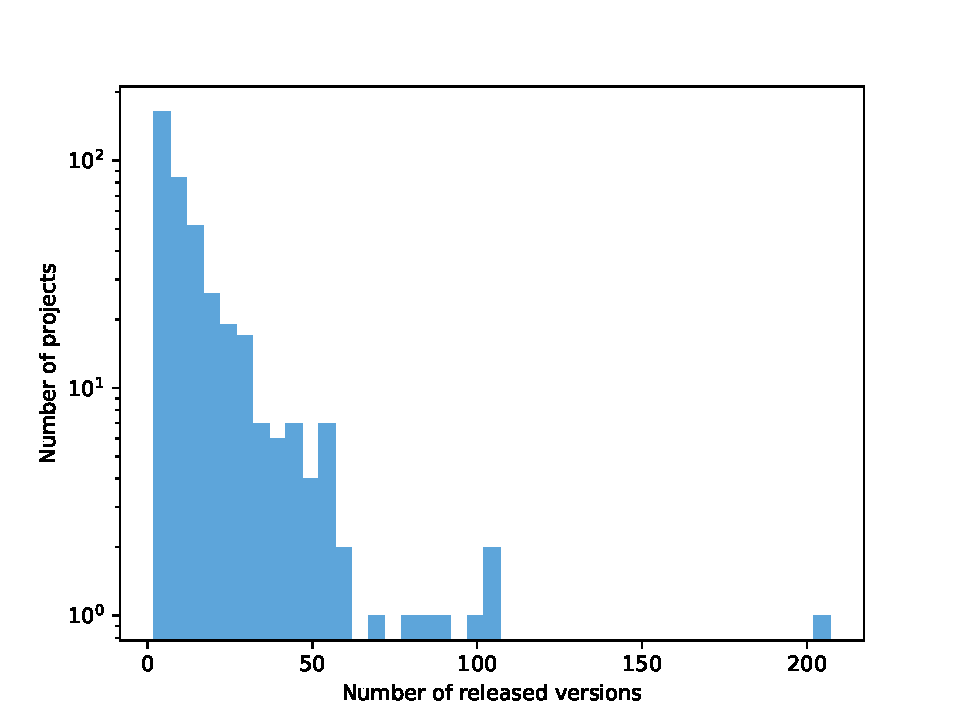
\includegraphics[height=0.4\textheight]
{images/evaluation/distribution_all_versions}
\end{figure}

\begin{figure}[]
\caption{Distribution of largest major versions}
\label{DistributionLargestMajor}
\centering
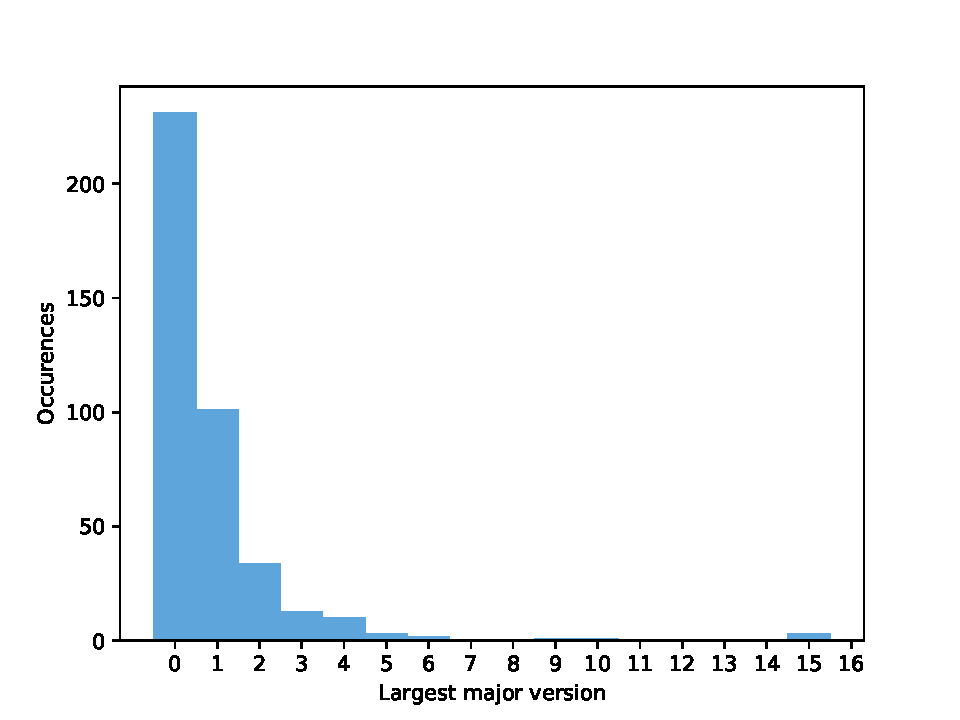
\includegraphics[height=0.4\textheight]
{images/evaluation/distribution_major_versions}
\end{figure}

\begin{figure}[]
\centering
\caption{Data sets}
\label{Datasets}
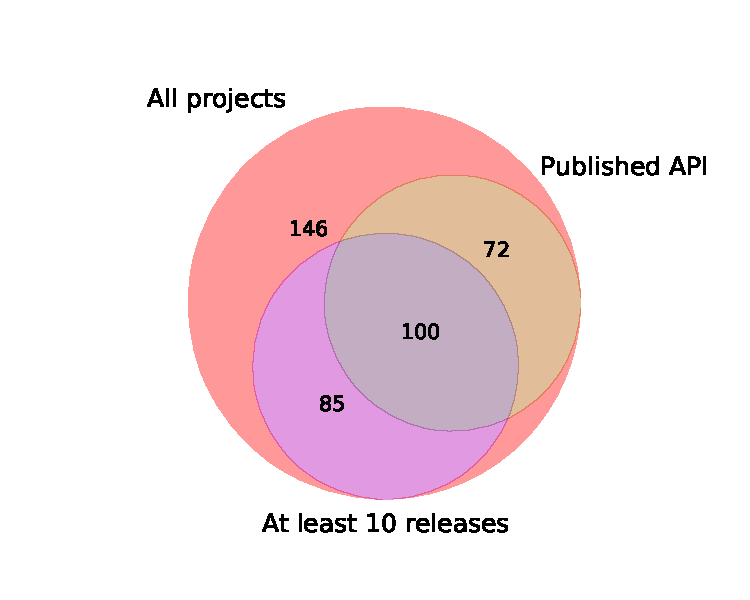
\includegraphics[height=0.4\textheight]
{images/evaluation/datasets}
\end{figure}

\begin{figure}[]
\centering
\caption{Percentage of total mismatches across projects (w/o structural
typing)}
\label{BoxplotsMismatches}
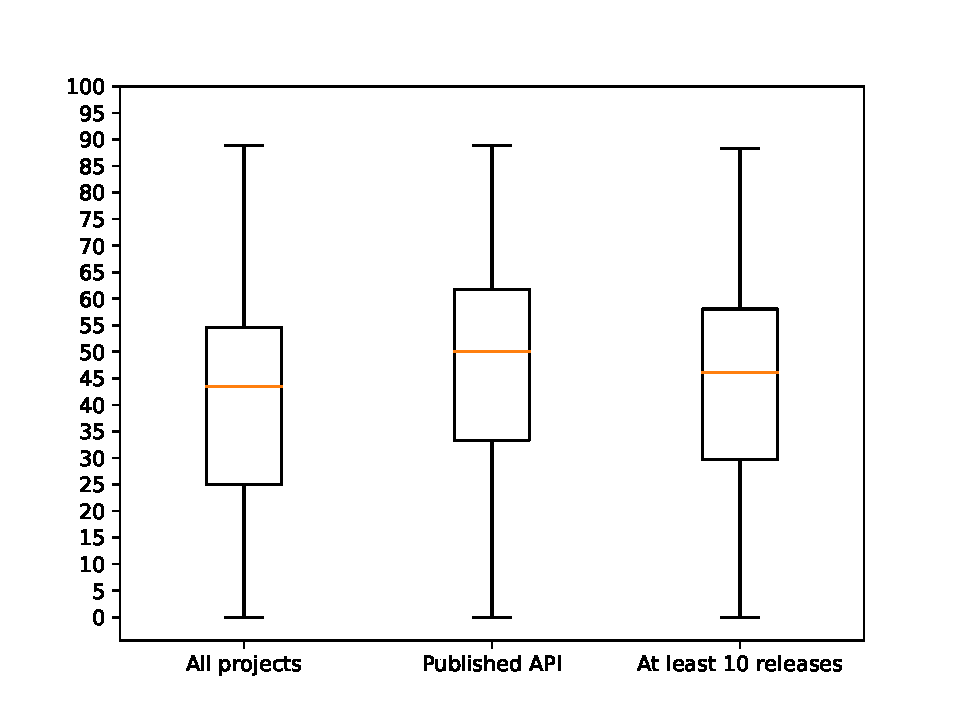
\includegraphics[height=0.4\textheight]
{images/evaluation/boxplots_mismatches}
\end{figure}

\begin{figure}[]
\centering
\caption{Percentages of breaking mismatches across projects (w/o
structural typing)}
\label{BoxplotsBreaking}
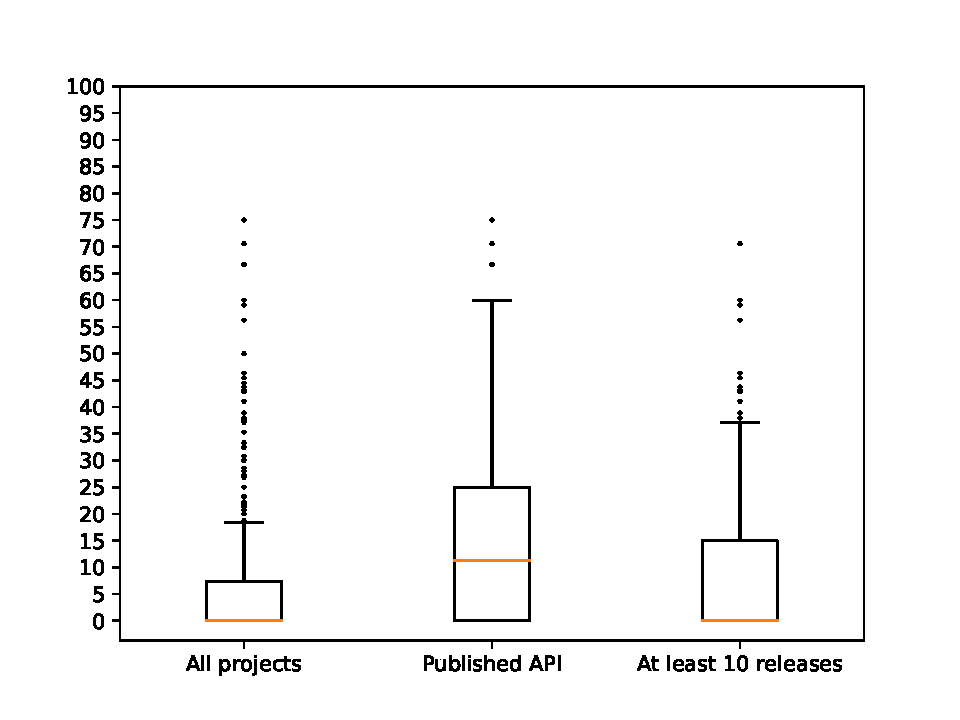
\includegraphics[height=0.4\textheight]
{images/evaluation/boxplots_breaking}
\end{figure}

\begin{figure}[]
\centering
\caption{Distribution of percentage of mismatches across projects with
a published API (w/o structural typing)}
\label{DistributionPublishedAPI}
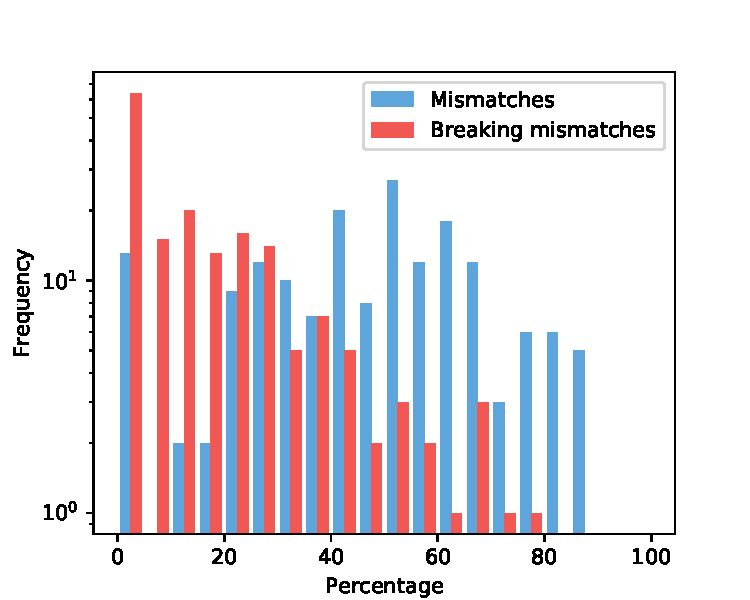
\includegraphics[height=0.4\textheight]
{images/evaluation/distribution_mismatches_major_version_1}
\end{figure}

\begin{figure}[]
\centering
\caption{Distribution of percentage of mismatches across projects with
more than 10 releases (w/o structural typing)}
\label{DistributionTenReleases}
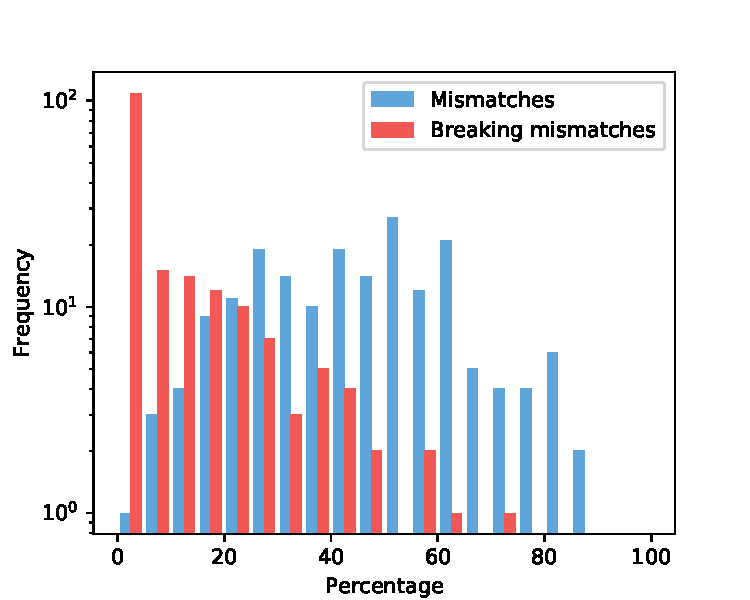
\includegraphics[height=0.4\textheight]
{images/evaluation/distribution_mismatches_more_than_10}
\end{figure}

\begin{figure}[]
\centering
\caption{Distribution of percentage of mismatches across all projects
(w/o structural typing)}
\label{DistributionAllProjects}
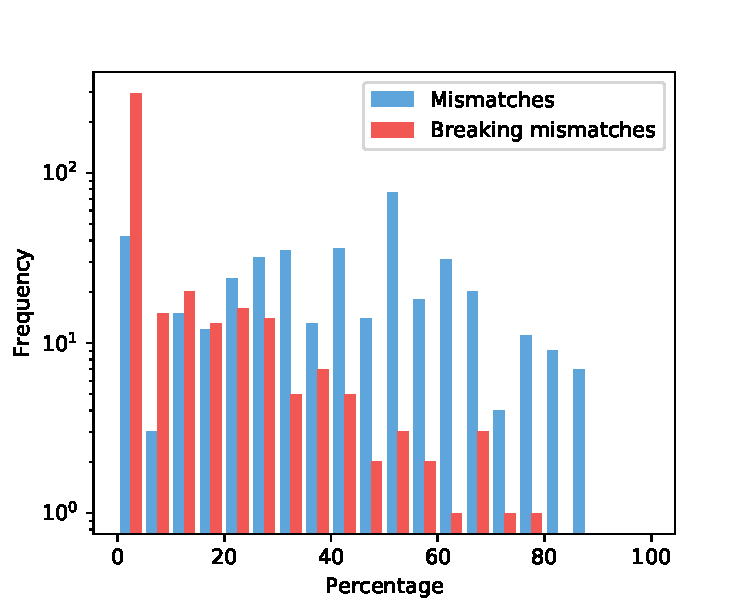
\includegraphics[height=0.4\textheight]
{images/evaluation/distribution_mismatches_all_projects}
\end{figure}

\begin{figure}[]
\centering
\caption{Histogram of total versions vs. breaking mismatches in a time
interval for all projects (w/o structural typing)}
\label{HistogramAllProjects}
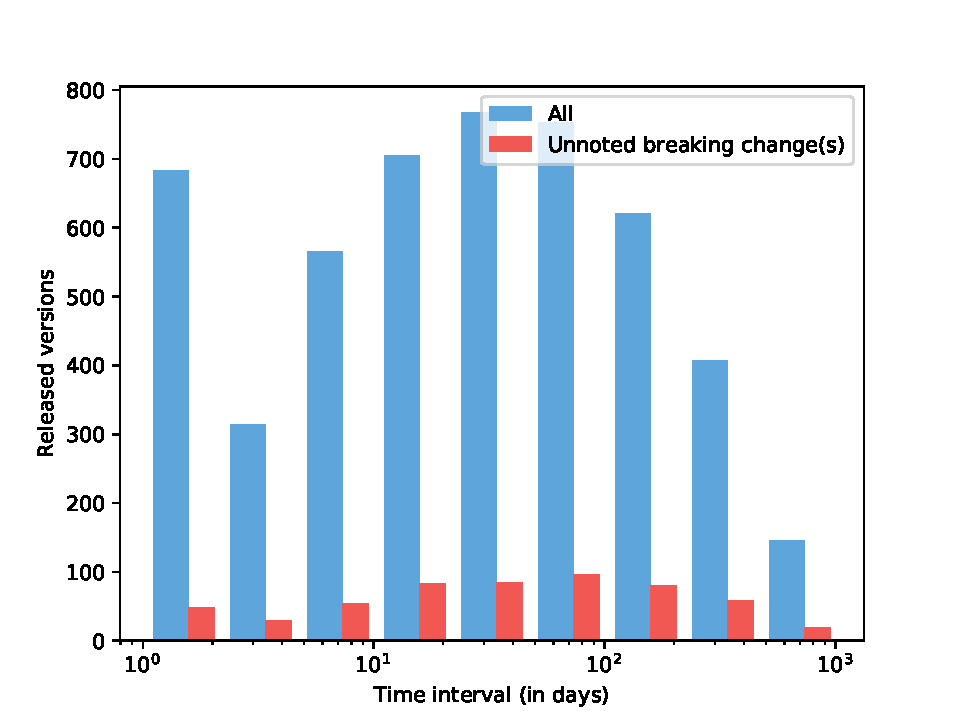
\includegraphics[height=0.4\textheight]
{images/evaluation/ls_nonstr_introduced_changes}
\end{figure}

\begin{figure}[]
\centering
\caption{Percentage of total mismatches across projects (w/ structural
typing)}
\label{StrBoxplotsMismatches}
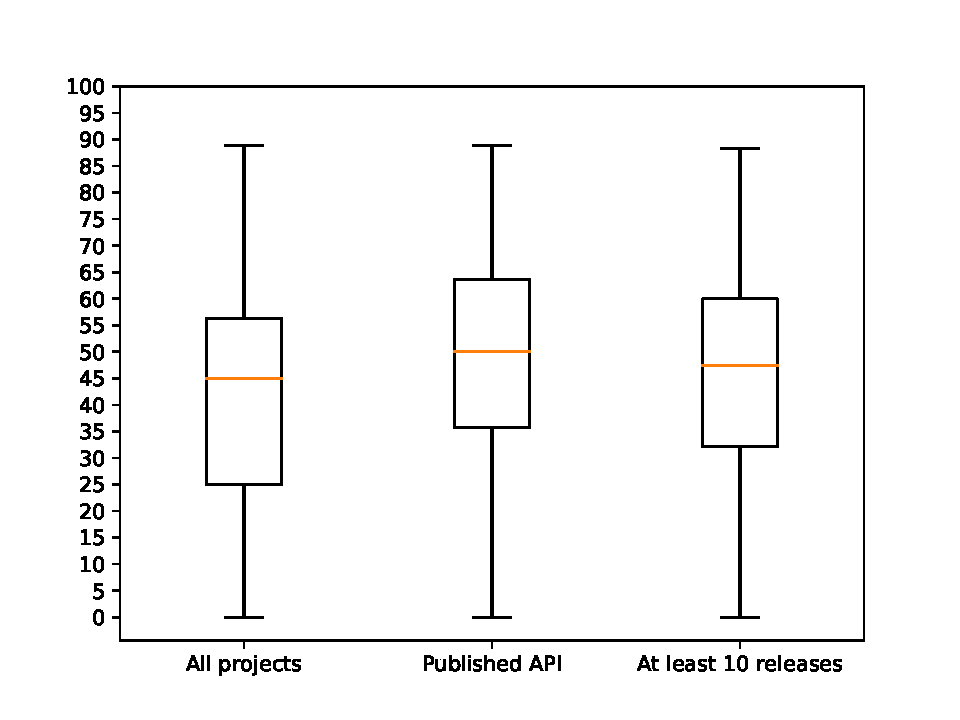
\includegraphics[height=0.4\textheight]
{images/evaluation/str_boxplots_mismatches}
\end{figure}

\begin{figure}[]
\centering
\caption{Percentages of breaking mismatches across projects (w/
structural typing)}
\label{StrBoxplotsBreaking}
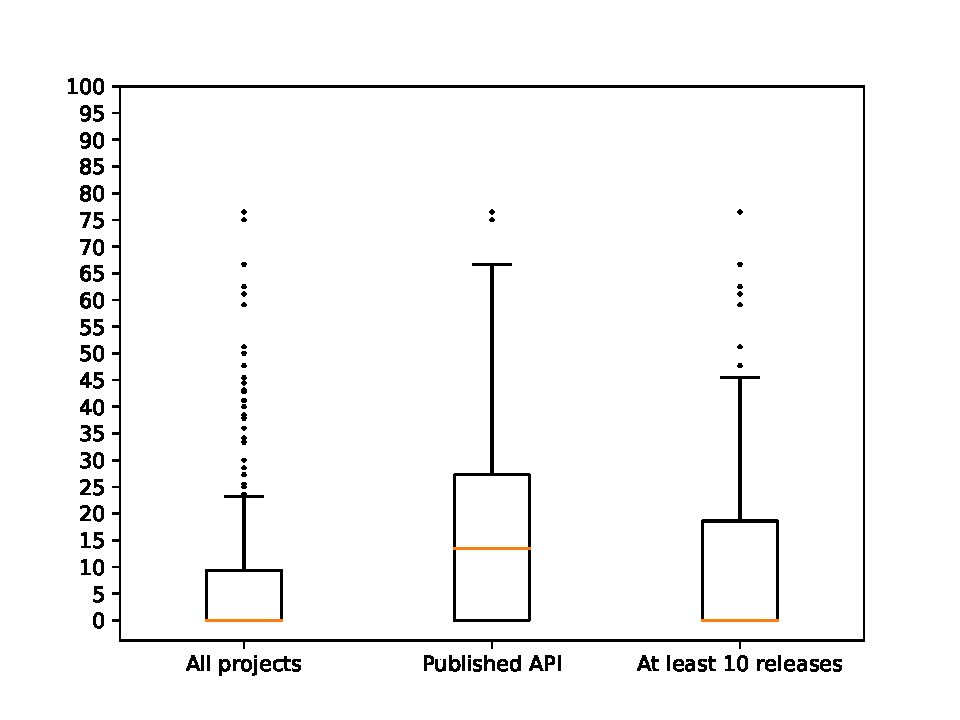
\includegraphics[height=0.4\textheight]
{images/evaluation/str_boxplots_breaking}
\end{figure}

\begin{figure}[]
\centering
\caption{Distribution of percentage of mismatches across projects with
a published API (w/ structural typing)}
\label{StrDistributionPublishedAPI}
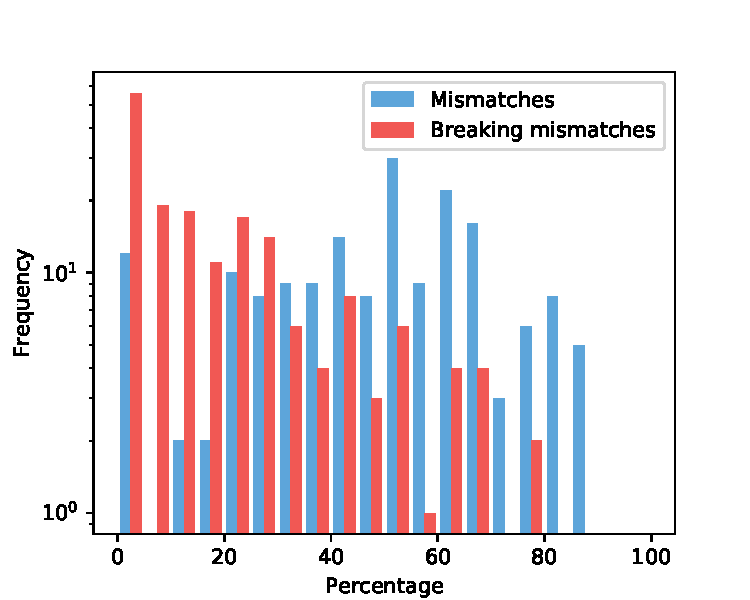
\includegraphics[height=0.4\textheight]
{images/evaluation/str_distribution_mismatches_major_version_1}
\end{figure}

\begin{figure}[]
\centering
\caption{Distribution of percentage of mismatches across projects with
more than 10 releases (w/ structural typing)}
\label{StrDistributionTenReleases}
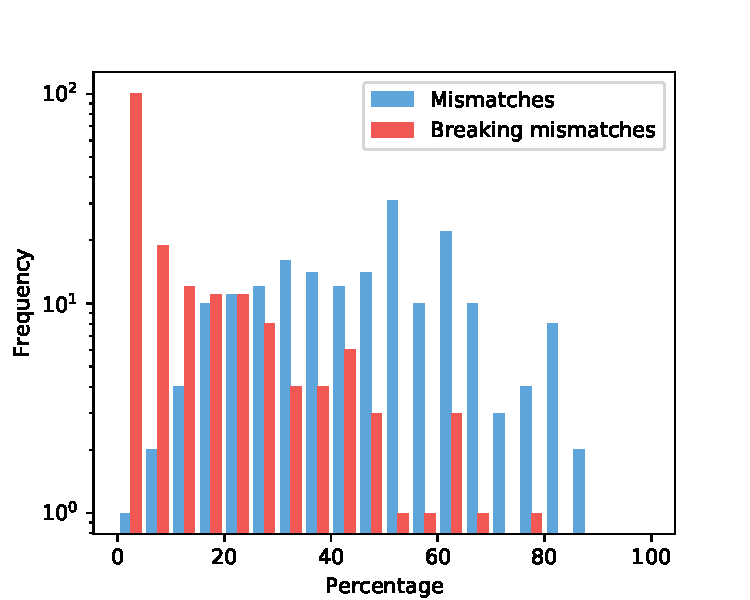
\includegraphics[height=0.4\textheight]
{images/evaluation/str_distribution_mismatches_more_than_10}
\end{figure}

\begin{figure}[]
\centering
\caption{Distribution of percentage of mismatches across all projects
(w/ structural typing)}
\label{StrDistributionAllProjects}
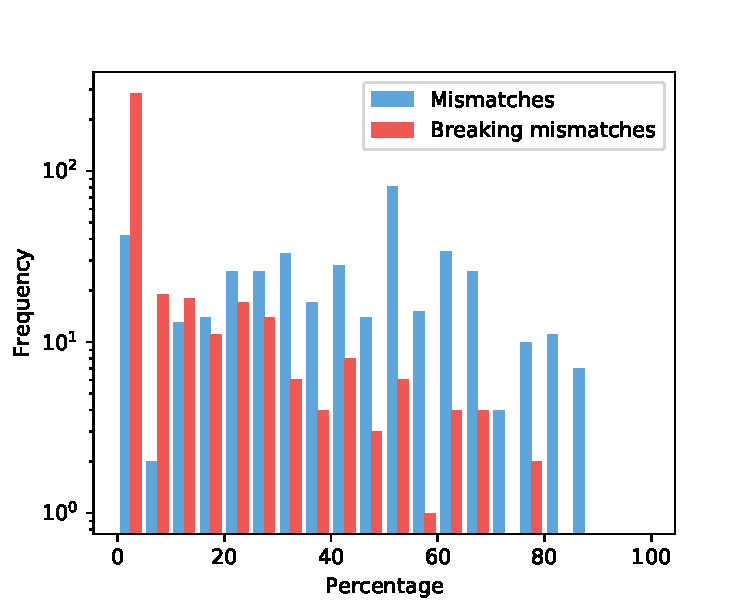
\includegraphics[height=0.4\textheight]
{images/evaluation/str_distribution_mismatches_all_projects}
\end{figure}

\begin{figure}[]
\centering
\caption{Histogram of total versions vs. breaking mismatches in a time
interval for all projects (w/ structural typing)}
\label{StrHistogramAllProjects}
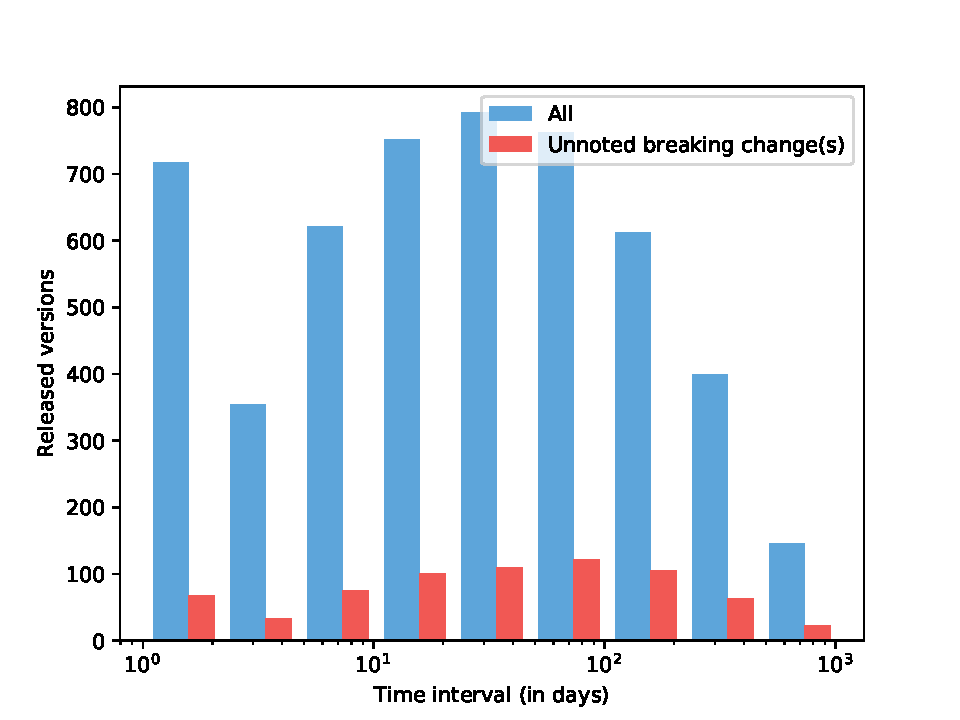
\includegraphics[height=0.4\textheight]
{images/evaluation/ls_str_introduced_changes}
\end{figure}

\end{appendices}

%=== Bibliography ===
\bibliographystyle{plain}
\bibliography{dissertation}

\end{document}

% This list of file-local variables enables
% auto filling of text and completely nukes all indentation
% except for code blocks.

% Local Variables:
% eval: (auto-fill-mode 1)
% sentence-end-double-space: nil
% LaTeX-indent-environment-list: (("verbatim" current-indentation) ("lstlisting" current-indentation))
% TeX-brace-indent-level: 0
% LaTeX-indent-level: 0
% LaTeX-item-indent: 0
% tex-indent-basic: 0
% tex-indent-item: 0
% tex-indent-arg: 0
% eval: (highlight-regexp "TODO")
% End:
